%--------------------------------------------------------------
% thesis.tex 
%--------------------------------------------------------------
% Corso di Laurea in Informatica 
% http://if.dsi.unifi.it/
% @Facolt\`a di Scienze Matematiche, Fisiche e Naturali
% @Universit\`a degli Studi di Firenze
%--------------------------------------------------------------
% - template for the main file of Informatica@Unifi Thesis 
% - based on Classic Thesis Style Copyright (C) 2008 
%   Andr\'e Miede http://www.miede.de   
%--------------------------------------------------------------
\documentclass[twoside,openright,titlepage,fleqn,
	headinclude,12pt,a4paper,BCOR5mm,footinclude]{scrbook}
%--------------------------------------------------------------
\newcommand{\myItalianTitle}{Algoritmi genetici e loro applicazioni\xspace}
\newcommand{\myEnglishTitle}{Genetic algorithms and their appplications\xspace}
% use the right myDegree option
\newcommand{\myDegree}{Corso di Laurea in Informatica\xspace}
%\newcommand{\myDegree}{
	%Corso di Laurea Specialistica in Scienze e Tecnologie 
	%dell'Informazione\xspace}
\newcommand{\myName}{Alessandro Ristori\xspace}
\newcommand{\myProf}{Maria Cecilia Verri\xspace}
%\newcommand{\myOtherProf}{Correlatore\xspace}
\newcommand{\mySupervisor}{Nome Cognome\xspace}
\newcommand{\myFaculty}{
	Scuola di Scienze Matematiche, Fisiche e Naturali\xspace}
\newcommand{\myUni}{\protect{
	Universit\`a degli Studi di Firenze}\xspace}
\newcommand{\myLocation}{Firenze\xspace}
\newcommand{\myTime}{Anno Accademico 2018-2019\xspace}
\newcommand{\myVersion}{Version 0.1\xspace}
%--------------------------------------------------------------
\usepackage[italian]{babel}
\usepackage[latin1]{inputenc} 
\usepackage[T1]{fontenc} 
\usepackage[square,numbers]{natbib} 
\usepackage[fleqn]{amsmath}  
\usepackage{ellipsis}
\usepackage{listingsutf8}
\usepackage{subfig}
\usepackage{caption}
\usepackage{appendix}
\usepackage{siunitx}
\usepackage{float}
\usepackage{color}
\usepackage{amsfonts}
\usepackage{array}
\usepackage{color, colortbl}
\usepackage{multirow}
%\usepackage[table]{xcolor}
\newcolumntype{L}[1]{>{\raggedright\arraybackslash}p{#1}}
\newcolumntype{C}[1]{>{\centering\arraybackslash}p{#1}}
\newcolumntype{R}[1]{>{\raggedleft\arraybackslash}p{#1}}
%\setlength{\extrarowheight}{3pt}
\definecolor{mygray}{rgb}{0.5,0.5,0.5}
%\usepackage{subcaption}
%\usepackage[framed,numbered,autolinebreaks,useliterate]{mcode}
%\usepackage[numbered,framed]{matlab-prettifier}
%\usepackage{matlab-prettifier}
%\usepackage[utf8]{inputenc}
%--------------------------------------------------------------
\usepackage{dia-classicthesis-ldpkg}
%--------------------------------------------------------------
% Options for classicthesis.sty:
% tocaligned eulerchapternumbers drafting linedheaders 
% listsseparated subfig nochapters beramono eulermath parts 
% minionpro pdfspacing
\usepackage[eulerchapternumbers,linedheaders,subfig,beramono,eulermath,
parts]{classicthesis}
%--------------------------------------------------------------
\newlength{\abcd} % for ab..z string length calculation
% how all the floats will be aligned
\newcommand{\myfloatalign}{\centering} 
\setlength{\extrarowheight}{3pt} % increase table row height
\captionsetup{format=hang,font=small}
%--------------------------------------------------------------
% Layout setting
%--------------------------------------------------------------
\usepackage{geometry}
\geometry{
	a4paper,
	ignoremp,
	bindingoffset = 1cm, 
	textwidth     = 13.5cm,
	textheight    = 21.5cm,
	lmargin       = 3.5cm, % left margin
	tmargin       = 4cm    % top margin 
}

\lstdefinestyle{default}{
  	frame=tb,
	language=Matlab,
  	aboveskip=3mm,
  	belowskip=3mm,
  	showstringspaces=false,
  	columns=flexible,
  	basicstyle={\small\ttfamily},
  	numbers=none,
  	breaklines=true,
  	breakatwhitespace=true,
  	tabsize=3
}
%--------------------------------------------------------------
\begin{document}
\frenchspacing
\raggedbottom
\pagenumbering{roman}
\pagestyle{plain}
%--------------------------------------------------------------
% Frontmatter
%--------------------------------------------------------------
%--------------------------------------------------------------
% titlepage.tex (use thesis.tex as main file)
%--------------------------------------------------------------
\begin{titlepage}
	\begin{center}
   	\large
      \hfill
      \vfill
      \begingroup
         
\includegraphics[scale=0.15]{logo/LOGO}\\
%			\spacedallcaps{\myUni} \\ 
			\myFaculty \\
			\myDegree \\ 
			\vspace{0.5cm}
         \vspace{0.5cm}    
         Tesi di Laurea    
      \endgroup 
      \vfill 
      \begingroup
      	\color{Maroon}\spacedallcaps{\myItalianTitle} \\ $\ $\\
      	\spacedallcaps{\myEnglishTitle} \\ 	
	\bigskip
      \endgroup
      \spacedlowsmallcaps{\myName}
      \vfill 
      \vfill
      Relatore: \emph{Maria Cecilia Verri}\\
      %Correlatore: \emph{Correlatore}\\
      \vfill
      \vfill
      \myTime
      \vfill                      
	\end{center}        
\end{titlepage}   
%--------------------------------------------------------------
% back titlepage
%--------------------------------------------------------------
   \newpage
	\thispagestyle{empty}
	\hfill
	\vfill
	\noindent\myName: 
	\textit{\myItalianTitle,} 
	\myDegree, \textcopyright\ \myTime
%--------------------------------------------------------------
% back titlepage end
%--------------------------------------------------------------
\pagestyle{scrheadings}
%--------------------------------------------------------------
% Mainmatter
%--------------------------------------------------------------
\pagenumbering{arabic}
% use \cleardoublepage here to avoid problems with pdfbookmark
%\include{intro} % use \myChapter command instead of \chapter
\tableofcontents
\listoffigures
\listoftables
\cleardoublepage
\thispagestyle{empty}
%\cleardoublepage
\begin{flushright}
\null\vspace{\stretch {1}}
\emph{"Possiamo vedere solo poco davanti a noi, ma possiamo vedere tante cose che bisogna fare." \break --- Alan Turing} \vspace{\stretch{2}}\null
\end{flushright}
\cleardoublepage
%\include{esercizi}

\myChapter{Introduzione}
%\section{Panoramica}
%Negli ultimi anni, grazie all'avvento e alla ribalta di nuove discipline e orizzonti per l'informatica come il machine learning e l'intelligenza artificiale, stanno ritornando in auge gli algoritmi genetici. La loro nascita si attesta negli anni '60 da parte di un team di ricerca il cui erede spirituale, oltre che pietra miliare in tale campo, sta nella figura di Goldman.\breakGli algoritmi genetici (che da ora in poi chiameremo GA per semplicità).
Il sempre maggiore interesse verso il machine learning, congiuntamente alla crescita esponenziale dell'importanza dell'intelligenza artificiale,  hanno riportato alla luce gli algoritmi genetici introdotti per la prima volta da J. Holland nel 1960 ed ampliamente analizzati dal successore di costui, D. E. Goldeberg \cite{goldberg1} nel 1989. Tali algoritmi stanno ritornando in auge grazie alla loro semplice implementazione ed alla loro adattablit\`a, il tutto combinato alla loro robustezza nel trovare la soluzione ottimale ad un problema di ricerca e/o ottimizzazione.

%\section{Seconda sezione}
%Testo.
Gli algoritmi genetici sono basati sui meccanismi della selezione naturale implementando scambi di informazioni casuali e deterministici combinati alla sopravvivenza degli "individui" pi\`u idonei; seppur l'idea su cui essi hanno le fondamenta e la loro implementazione siano relativamente pi\`u semplici rispetto ai metodi tradizionali, lo studio degli algoritmi genetici non \`e assolutamente meno degno di nota.
\vspace{3mm}

Lo scopo che si prefigge questa tesi \`e dare una visione precisa del funzionamento degli algoritmi genetici e delle loro caratteristiche peculiari, il tutto supportato tramite esempi pratici e, al tempo stesso, metterne in luce i vantaggi e gli svantaggi che ne derivano; da qui in avanti ci riferiremo agli algoritmi genetici con l'acronimo, proveniente dall'inglese, GA.

La tesi, dopo questa prima introduzione, \`e strutturata nel seguente modo:
\begin{enumerate}
%\setcounter{enumerate}{2}
    \item Il capitolo 2, dopo una breve introduzione storica, tratta nel dettaglio i principi fondamentali dei GA ed il loro funzionamento, illustrando le funzioni che li caratterizzano come tali.
    \item Il capitolo 3 porta un esempio semplice di applicazione di un GA, oltre ad evidenziare svantaggi e vantaggi di questo approccio.
    %\item Il capitolo 4 illustra il funzionamento di un GA con il compito di ordinare un array confrontando le sue prestazioni con i pi\`u famosi algoritmi di ordinamento.
    \item Il capitolo 4 illustra il problema del cammino minimo in un grafo con annesso riferimento all'algoritmo di Dijkstra, in seguito mostra il lavoro eseguito dal GA costruito per lo stesso compito; per ultimo, i due algoritmi vengono messi a confronto con maggiore approfondimento dei pro e contro del GA in tale problema ed affini.
    \item Il capitolo 5 discute su quanto visto nei capitoli precedenti, arrivando a conclusioni volte a migliorare gli esempi di implementazioni illustrati. Al tempo stesso, daremo una visione pi\`u ampia sui campi di applicazione dei GA, mostrando come essi stiamo attirando un sempre maggiore interesse, concludendo il tutto con una visione sul futuro di tale approccio.
    \item Dopo i necessari ringraziamenti, al termine della tesi (in un'apposita appendice) si potranno osservare i codici usati nell'arco di tutti i capitoli della tesi.
    %\item Il capitolo 5 tratta dell'uso dei GA con i grafi (colorazione, ricerca del cammino minimo, etc...), con una parentesi riguardo il problema del commesso viaggiatore.
    %\item Il capitolo 6, in conclusione, mostra la risoluzione di sudoku attraverso i GA e l'importanza di tutto questo.
\end{enumerate}
\newpage
%\cleardoublepage

\myChapter{Storia, Principi ed Operatori dei GA}
Nel seguente capitolo introdurremo gli algoritmi genetici mostrando brevemente la loro storia; per capire il principio su cui essi sono stati fondati e le loro caratteristiche peculiari ci baseremo su quanto scritto da Goldberg \cite{goldberg1} nella sua opera maggiormente conosciuta.
\section{Nascita e Principio}
Gli algoritmi genetici, pi\`u conosciuti nel mondo scientifico come GA, sono algoritmi di ricerca ed ottimizzazione introdotti per la prima volta da John Holland e dai suoi colleghi all'universit\`a del Michigan all'inizio degli anni '60, ed in seguito profondamente analizzati da David E. Goldberg nel suo libro "Genetic Algorithms in Search, Optimization \& Machine Learning" pubblicato nel 1989. Gli obiettivi principali della ricerca portata avanti da Holland e Goldberg sono stati in primo luogo astrarre e spiegare in modo rigoroso i processi adattativi dei sistemi naturali e, di conseguenza, costruire sistemi software in grado di conservare i meccanismi di tali sistemi.
\vspace{3mm}

I GA, com'\`e possibile dedurre dal loro nome, si basano sul principio darwiniano della sopravvivenza e riproduzione degli individui pi\`u idonei, attraverso lo scambio casuale, ma pur sempre strutturato, di informazioni volto alla creazione di algoritmi adattibili ad un'ampia  classe di problemi. Ad ogni generazione vengono creati nuovi individui a partire dai migliori di quelle precedenti ed i peggiori vengono rimpiazzati secondo logiche ben precise; al termine della riproduzione vengono valutati i vari individui, ai quali viene assegnato un valore di idoneit\`a, necessario per lo sviluppo delle successive generazioni.

La grande sfida che la ricerca sugli algoritmi genetici si pone \`e la \textit{robustezza}, ovvero l'equilibrio fra efficienza ed efficacia necessario per la riuscita, sopravvivenza e miglioramento nei vari ambiti di applicazione dei GA; la robustezza implica una diminuzione, o la totale eliminazione, dei costi di re-design di un sistema e maggiore \`e essa pi\`u a lungo ed in modo migliore i sistemi potranno comportarsi. \`E meraviglioso accorgersi di come il parametro della robustezza sia presente ovunque nei sistemi naturali, nei quali vigono regole di auto-miglioramento, auto-riparazione e riproduzione attraverso le meccaniche della selezione naturale; questo meccanismo \`e praticamente sconosciuto nel mondo dei sistemi artificali, ma \`e prorio qui che entrano in scena i GA.
\section{Caratteristiche Peculiari}
Secondo quanto stabilito da Goldberg in \cite{goldberg1}, nella ricerca della robustezza i GA differiscono molto dalle pi\`u note procedure di ricerca ed ottimizzazione particolarmente per quattro motivi:
\begin{enumerate}
    \item I GA lavorano tramite codifiche di un insieme di parametri, non con i parametri stessi.
    \item I GA cominciano la loro ricerca da una popolazione di punti, non da uno solo.
    \item I GA usano una funzione oggettiva per la valutazione delle informazioni ottenute, non hanno bisogno di dati ausiliari.
    \item I GA usano regole dettate dalla probabilit\`a, non sono deterministici.
\end{enumerate}
Come si pu\`o osservare dal primo punto elencato, gli algoritmi genetici hanno bisogno che l'insieme di parametri di un problema di ricerca e/o ottimizzazione sia codificato come un insieme di stringhe definite su un alfabeto finito.

Consideriamo, come fatto da Goldberg stesso nella sua opera \cite{goldberg1}, una scatola chiusa con sette interruttori che agiscono da input, per ogni combinazione esiste un segnale di output f che in termini matematici pu\`o essere espresso come f(i), dove i \`e una qualunque combinazione dei sette interrutori; l'obiettivo del problema consiste nell'impostare gli interruttori in modo da ottenere il massimo valore che f pu\`o assumere; con i GA per prima cosa codifichiamo gli interruttori stessi come una stringa: la soluzione pi\`u semplice prevede di implementare una stringa di sette valori binari dove l'1 rappresenta il segnale ON e lo 0 il segnale OFF: per esempio la stringa 1001110, rappresenta la combinazione in cui il secondo, il terzo e l'ultimo interruttore sono spenti.
\begin{figure}[H]
    \centering
    \hfill
    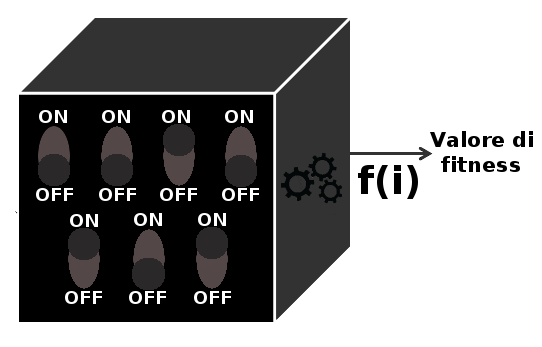
\includegraphics[width=0.85\textwidth]{Images/immagine1.png}
    \hspace*{\fill}
    \caption{I GA hanno bisogno solamente di una codifica e di una funzione di fitness per il loro funzionamento, a loro non interessano i meccanismi interni al problema.}
    \label{fig:box_switches}
\end{figure}
Come suggerito dal punto 2, gli algoritmi genetici cominciano con una popolazione di invidividui (in questo caso, stringhe) e da esse vengono prodotte le generazioni successive, nel problema preso in considerazione una combinazione casuale di partenza potrebbe essere data dal lancio di una moneta (testa == $1$, croce == $0$) con dimensione delle popolazione uguale a 5 (cifra molto esigua per gli standard dei GA):\vspace{3mm}
\break
$1010110\break
0001101\break
1100010\break
1110101\break
0010001$\vspace{3mm}

Dopo di ci\`o, le successive popolazioni sono generate attraverso i vari passi dell'algoritmo genetico (andremo nel dettaglio nella prossima sezione), il quale non richiede altre informazioni per operare, di fatto si potrebbe dire che i GA sono \textit{ciechi}: per raggiungere il loro obiettivo hanno solo bisogno di un valore di payoff associato ad ognuna delle stringhe della popolazione, nel caso da noi preso in esame altro non \`e che la funzione f(i). Questo rende l'approccio coi GA molto pi\`u semplice rispetto ai suoi concorrenti, ma, d'altro canto, il rifiuto di usare conoscenze specifiche laddove possibile potrebbe limitare le performance di un GA nel caso si trovasse faccia a faccia con metodi specifici per un dato problema.
\vspace{3mm}

Il punto 4, per concludere, sottolinea che i GA usano regole probabilistiche per guidare la propria ricerca, questo potrebbe far storcere il naso a molti, dato che siamo abituati a lavorare per la maggior parte del nostro tempo con metodi deterministici; l'uso della probabilit\`a non implica che i GA siano un semplice metodo di ricerca fondato sulla pura casualit\`a: la presa di una decisione non avviene tramite il semplice lancio di una moneta, la ricerca \`e di fatto guidata verso la soluzione migliore; \textit{la probabilit\'a svolge soltanto un ruolo di strumento necessario per l'attuazione}.

Prese in considerazione le quattro differenze elencate all'inizio di questa sezione, entreremo maggiormente in dettaglio nell'esecuzione di un algoritimo genetico nella prossima sezione attraverso la dettagliata descrizione delle sue funzioni principali.
\section{Glossario ed Operatori Fondamentali}
I meccanismi di un GA sono estremamente semplici, in quanto si basano nientemeno che sulla copia di stringhe e sullo scambio di sottostringhe, ma la ragione per cui questo processo non risulta arduo \`e ancora pi\`u sottile e potente; la facilit\`a delle operazioni da eseguire sulle stringhe e la loro efficacia sono i maggiori punti di forza dei GA.
\vspace{3mm}

Prima di addentrarci nella descrizione dei meccanismi di un GA occorre introdurre i termini \cite{goldberg1}, derivanti in gran parte dalla biologia, che ci accompagneranno per tutta la tesi:
\begin{enumerate}
    \item \textbf{Cromosoma}; codifica di una delle soluzioni al problema preso in esame, rappresentato come una stringa numerica/alfanumerica a seconda del contesto. La lunghezza delle stringa \`e strettamente correlata al problema (si noti l'esempio portato nella sezione 2.2).
    \item \textbf{Popolazione}; insieme di individui, quest'ultimi rappresentati da cromosomi e, dunque, altro non \`e che il set complessivo delle soluzioni ad un problema.
    \item \textbf{Gene}; parte di un cromosoma, corrispondente ad un elemento della stringa.
    \item \textbf{Allele}; il valore che un gene pu\`o assumere, nel caso di stringhe binarie gli alleli sono $0$ ed $1$.
    \item \textbf{Locus}; posizione di un gene nella stringa, nella maggioranza dei casi useremo questo termine con lo stesso significato di gene.
    \item \textbf{Fitness o Idoneit\`a}; grado di idoneit\`a di una particolare soluzione al problema dato. Tale valore \`e generato da un'apposita \textit{funzione di fitness} ad hoc.
\end{enumerate}
Armati di questi termini possiamo, a questo punto, vedere nel dettaglio gli operatori (le cui innumerevoli varianti sono state approfonditamente illustrate in \cite{glossary}) che definiscono i GA come tali.
\subsection{Selezione}
Operatore conosciuto anche come \textit{riproduzione}, \`e un processo nel quale le stringhe di una data popolazione sono copiate rispetto al valore obiettivo di una funzione di fitness f, la quale pu\`o essere vista (nei casi noti della vita di tutti i giorni) come una misura di un profitto od utilit\`a che desideriamo massimizzare.
Copiare le stringhe a seconda del loro valore di fitness comporta una maggiore probabilit\`a, per quelle stringhe che hanno ottenuto i pi\`u alti risultati, di contribuire alla generazione della prossima popolazione.

La selezione altro non \`e che la versione artificiale del pi\`u famoso meccanismo darwiniano della selezione naturale: in quest'ultimo caso il fitness di una popolazione proviene dalle capacit\`a di sopravvivenza di una specie, mentre nel nostro sistema artificiale \`e dato da una funzione oggettiva che determina la vita o la morte di una stringa.
\vspace{3mm}

L'operatore di selezione pu\`o essere implementato in forma algoritmica in base a numerose tecniche \cite{glossary} \cite{selection2}, di seguito sono presentate quelle pi\`u conosciute:
\begin{itemize}
    \item \textbf{Casuale:} forma pi\`u semplice in assoluto, ma meno efficiente; data una popolazione di dimensione N, una stringa ha probabilit\`a di riproduzione pari a \(\frac{1}{N}\).
    \item \textbf{A roulette:} sia N la dimensione della popolazione e \(f\ped{i}\) il valore di fitness dell'i-esima stringa, allora la probabilit\`a con la quale essa potrebbe essere scelta corrisponde a: $$p\ped{i}=\frac{f\ped{i}}{\sum_{j=1}^{N} f\ped{j}}$$
    \item \textbf{Rapportato al migliore:} siano N ed f\ped{i} definiti come in precedenza e sia f\ped{M} il valore massimo di fitness ottenuto ad una determinata generazione, un individuo pu\`o essere selezionato con probabilit\`a: $$p\ped{i}=\frac{f\ped{i}}{f\ped{M}}$$In questo caso l'individuo migliore sar\`a sempre in grado di partecipare al crossover.
    \item \textbf{A categoria:} simile alla prima, ma vengono considerate tutte le coppie possibili di individui, computazionalmente non efficiente dato che potrebbe trovarsi in stallo nel caso in cui ci fossero due coppie con valori di fitness molto vicine fra loro.
    \item \textbf{A torneo \cite{selection1}:} prevede lo svolgimento di "tornei" fra pochi cromosomi scelti in modo casuale dalla popolazione; il vincitore di ciascun "torneo" \`e scelto per il crossover, pi\`u la dimensione del torneo \`e maggiore meno probabile sar\`a la scelta di un individuo con fitness bassa, dato che aumentano le possibilit\`a che un cromosoma con alta fitness partecipi al torneo.
    
    L'algoritmo funziona pressapoco nel seguente modo:
    \begin{enumerate}
        \item seleziona k (dimensione del torneo) individui dalla popolazione in modo casuale;
        \item scelta del miglior cromosoma dal torneo con probabilit\`a p;
        \item scelta del secondo miglior cromosoma con probabilit\`a $$p*(1-p)$$
        \item scelta del terzo miglior cromosoma con  probabilit\`a $$p*(1-p)^2$$
        \item scelta dell'iesimo miglior cromosoma con probabilit\`a $$p*(1-p)^{(i-1)}$$ e cos\`i via fino a raggiungere il k-esimo elemento;
    \end{enumerate}
    Rispetto alle precedenti forme, la selezione a torneo risulta pi\`u semplice e lavora efficaciemente su architetture parallele, oltre ad essere indipendente da funzioni di fitness scalari; si noti che con k=1 si ottiene una selezione casuale.
\end{itemize}
\subsection{Crossover}
L'operatore di crossover si occupa dello scambio di informazioni fra due individui della popolazione che hanno superato la fase di selezione con l'obiettivo di produrre prole, la quale potrebbe avvicinarsi alla soluzione richiesta. 
Prendiamo come esempio il crossover semplice (scelta casuale di due individui che hanno superato la selezione attraverso l'apposito operatore) e mostriamo come esegue il proprio compito.%il quale non \`e detto che avvenga ad ogni iterazione del GA (esiste una frequenza di crossover p\ped{c}), e mostriamo come esso esegue il proprio lavoro.
\vspace{3mm}

Se l \`e la dimensione dei cromosomi, sia k intero scelto in modo casuale nell'intervallo [1, l-1] e rappresentante il \textit{punto di crossover} da cui due individui si scambieranno i propri geni; lo scambio avviene, nella variante pi\`u semplice, fra le posizioni [k+1, l] e da esso saranno generati due nuovi cromosomi. Per avere un'idea migliore del funzionamento, mostriamo i vari tipi di crossover con annessa figura esplicativa:
\begin{itemize}
    \item\textbf{Casuale:} per ciascuna coppia di geni viene generato un numero intero fra $0$ ed $1$, se il numero risulta $1$ allora il cromosoma figlio erediter\`a il gene del primo individuo, altrimenti riceve il gene dal secondo. Questa forma di crossover distribuisce in modo casuale i geni dei genitori, risulta la meno efficiente fra quelle esposte.
    \begin{figure}[H]
        \centering
        \hfill
        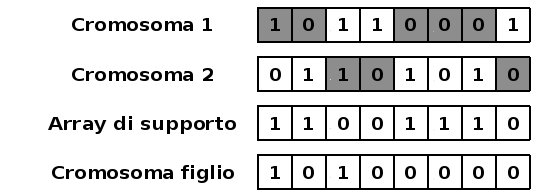
\includegraphics[width=0.95\textwidth]{Images/CrossoverRandom.png}
        \hspace*{\fill}
        %\caption{I GA hanno bisogno solamente di una codifica e di una funzione di fitness per il loro funzionamento, a loro non interessano i meccanismi interni al problema.}
        \caption{Crossover casuale}
        \label{fig:randomcrossover}
    \end{figure}
    \item \textbf{A punto singolo:} variante spiegata nel breve esempio introduttivo, gli array rappresentanti i cromosomi vengono "tagliati" ad un punto di crossover k, determinato in modo casuale o predefinito; il primo figlio sar\`a dato dalla combinazione dei primi k geni del primo individuo e dai restanti l-k geni del secondo, il secondo figlio sar\`a generato in modo quasi simmetrico (testa del secondo cromosoma e coda del primo).
    \begin{figure}[H]
        \centering
        \hfill
        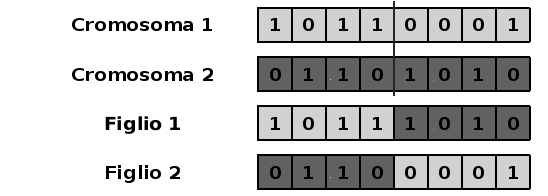
\includegraphics[width=0.95\textwidth]{Images/CrossoverSinglePoint.png}
        \hspace*{\fill}
        %\caption{I GA hanno bisogno solamente di una codifica e di una funzione di fitness per il loro funzionamento, a loro non interessano i meccanismi interni al problema.}
        \caption{Crossover a punto singolo}
        \label{fig:singlepointcrossover}
    \end{figure}
    \item \textbf{A punto doppio:} variante del precedente, vi sono, come dice il nome, due punti di crossover k e j, la figura 4 mostra molto semplicemente il suo funzionamento.
    \begin{figure}[H]
        \centering
        \hfill
        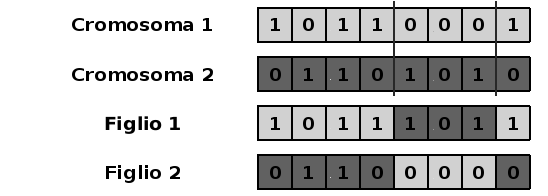
\includegraphics[width=0.95\textwidth]{Images/CrossoverDoublePoints.png}
        \hspace*{\fill}
        %\caption{I GA hanno bisogno solamente di una codifica e di una funzione di fitness per il loro funzionamento, a loro non interessano i meccanismi interni al problema.}
        \caption{Crossover a punto doppio}
        \label{fig:doublepointcrossover}
    \end{figure}
\end{itemize}
Per terminare la sezione, vorremmo far notare che il crossover fra due cromosomi, a differenza della selezione, non avviene ad ogni iterazione del GA, ma ha una frequenza pari a p\ped{c}, arbitrariamente scelta dal programmatore. 
\subsection{Mutazione}
L'ultimo operatore che caratterizza i GA consiste nella mutazione: nei sistemi naturali essa viene definita come un'anomalia nel corredo genetico di un individuo che potrebbe causare miglioramenti o peggioramenti nelle condizioni di vita, nei sistemi artificiali (nel nostro specifico interesse, nei GA) consiste nella modifica dei geni di cromosoma in base ad un coefficiente di mutazione p\ped{m} definito all'inizio del programma.
%\vspace{3mm}

La mutazione ha il compito di migliorare il valore di fitness di un individuo e/o ampliare lo spazio di ricerca nel problema, in modo da non cadere e rimanere in ottimi locali, punto di debolezza dei GA, di cui parlaremo in un apposito capitolo.

Passata una stringa all'operatore, quest'ultimo pu\`o cambiare ogni singolo gene con coefficiente p\ped{m}; \`e evidente il fatto che un valore troppo alto di p\ped{m} possa portare su una strada sbagliata il GA, mentre un valore estremamente basso non influisce in alcun modo sull'andamento dell'algoritmo.
\newpage
%\begin{thebibliography}{99}

\bibitem{goldberg1}{D. E. Goldberg - \emph{Genetic Algorithms in Search, Optimization \& Machine Learning} - Addison-Wesley, 1989}

\bibitem{selection1}{B. L. Miller, D. E. Goldberg - \emph{Genetic Algorithms, Tournament Selection, and the Effects of Noise} - Complex Systems, 9, 1995, Pages 193-212}

\bibitem{selection2}{R. Sivaraj, T. Ravichandran - \emph{A Rewiew of Selection Methods In Genetic Algorithm}}

\bibitem{glossary}{Thomas Baeck, D.B Fogel, Z Michalewicz - \emph{Evolutionary Computation 1: Basic Algorithms and Operators}}

\bibitem{path1}{Tony White, Bernard Pagurek, Franz Oppacher1 - \emph{ASGA: Improving the Ant System by Integration with Genetic
Algorithms} - altre informazioni}

\bibitem{path2}{Sachith Abeysundara, Baladasan Giritharan, Saluka Kodithuwakku - \emph{A Genetic Algorithm Approach to Solve the
Shortest Path Problem for Road Maps}}

\bibitem{path3}{Bilal Gonen - \emph{Genetic Algorithm Finding the Shortest Path in Networks}}

\bibitem{path4}{Yinzhen Li, Ruichun He, Yaohuang Guo - \emph{Faster Genetic Algorithm for Network Paths}}

\bibitem{tsp1}{Michael J\"unger, Gerhard Reinelt, Giovanni Rinaldi - \emph{Handbooks in Operations Research and Management Science} - Volume 7, 1995, Pages 225-330}

\bibitem{tsp2}{Heinrich Braun - \emph{On solving travelling salesman problems by genetic algorithms}}

\bibitem{tsp3}{H. M\"uhlenbein, M. Gorges-Schleuter, O. Kr\"amer - \emph{Evolution algorithms in combinatorial optimization} - Volume 7, Issue 1, April 1988, Pages 65-85}

\bibitem{tsp4}{Noraini Mohd Razali, John Geraghty
 - \emph{Genetic Algorithm Performance with Different
Selection Strategies in Solving TSP}}

\bibitem{tsp5}{P. Larranaga, C. M. H. Kuijpers, R. H. Murga, I. Inza, S. Dizdarevic - \emph{Genetic Algorithms for the Travelling Salesman Problem: A Review of Representations and Operators} -  Artificial Intelligence Review 13, 1999, Pages 129-170}

\bibitem{path5}{K. De Jong, W. M. Spears - \emph{Using Genetic Algorithms to Solve NP Complete Problems} - Proceedings of the Third International Conference on Genetic Algorithm, Morgan Kaufman, Los Altos, CA, 1989, Pages 124-132}

\bibitem{graphcol1}{Musa M. Hindi, Roman V. Yampolskiy - \emph{Genetic Algorithm Applied to the Graph Coloring Problem}}

\bibitem{graphcol4}{Josephine Yik Chong Leung, Wai Shan Lui - \emph{The Application of Graph Theory to Sudoku} - Hang Lung Mathematics Awards, 2014, Vol. 6}

\bibitem{graphcol2}{Timo Mantere, Janne Koljonen - \emph{Solving, rating and Generating Sudoku Puzzles with GA}}

\bibitem{graphcol3}{Bah-Hwee Gwee, Josep S. Chang - \emph{A hybrid genetic hill-climbing algorithm for four-coloring map problems} - Design and application of hybrid intelligent systems, 2003, Pages 252-261}

\bibitem{graphcol5}{Xiu Qin Deng, Yong Da Li - \emph{A novel hybrid genetic algorithm for solving Sudoku puzzles}}

\bibitem{graphcol6}{Charles Fleurent, Jacques A. Ferland - \emph{Genetic and hybrid algorithms for graph coloring} - Annals of Operations Research, June 1996, Volume 63, Issue 3, Pages 437-461}

\bibitem{end1}{H. Khayyam, A. Jamali, H. Assimi, R. N. Jazar (2020) - \emph{Genetic Programming Approaches in Design and Optimization of Mechanical Engineering Applications} - Nonlinear Approaches in Engineering Application, 2019, Pages 367-402}

\bibitem{end2}{Seyedali Mirjalil, Jin Song Dong, Ali Safa Sadiq, Hossam Faris - \emph{Genetic Algorithm: Theory, Literature Review, and Application in Image Reconstruction} - Nature-Inspired Optimizers, 2019, Pages 69-85}

\bibitem{end3}{S. K. Pal, P. P. Wang - \emph{Genetic algorithms for pattern recognition}}

\bibitem{end4}{John J. Grefenstette - \emph{Genetic Algorithms and Machine Learning}}

\bibitem{end5}{Haleh Vafaie, Kenneth De Jong
 - \emph{Genetic Algorithms as a Tool for Feature Selection in Machine Learning}}
 
\bibitem{end6}{Robert Pereira - \emph{Genetic Algorithm Optimisation for Finance and Investment} - 2000}

%\bibitem{graphcol5}{ - \emph{}}

%\bibitem{graphcol4}{ - \emph{}}

%\bibitem{tsp2}{}

\end{thebibliography}


\myChapter{Implementazione di un GA}
Nel seguente capitolo, prendendo spunto da quanto illustrato da Goldberg nel massimizzare una funzione \cite{goldberg1}, mostreremo una semplice implementazione di un GA, partendo dalla costruzione delle strutture dati e dalla applicazione degli algoritmi necessari al suo lavoro; pi\`u nello specifico, utilizzando MatLab ed osservando quanto fatto da Goldberg (seppure con le dovute modifiche), cercheremo di trovare il minimo di una funzione ponendo in mostra le varie fasi di lavoro ed alcuni problemi di implementazione che potrebbero sorgere nell'utilizzo di un GA.
\vspace{3mm}

Ci pare giusto evidenziare il fatto che Matlab implementa gi\`a di default un algoritmo genetico per l'ottimizzazione di funzioni (al tempo stesso ne sono stati sperimentati molti altri \cite{matlab3}) e che ulteriori lavori sono stati eseguiti da diversi esperti del settore e del linguaggio \cite{matlab1} \cite{matlab2}, il nostro compito consisteva nel rendere pi\`u comprensibile l'attuazione di un GA ed il flusso del codice che lo implementa.
\section{Le strutture dati e scelta dei coefficienti}
Gli algoritmi genetici lavorano con stringhe, perci\`o \`e naturale che la popolazione sia un insieme di esse, per l'implementazione del nostro GA di esempio ci baseremo su questo fatto: ogni individuo \`e rappresentato da un array binario, rappresentante i geni, di una dimensione in accordo col problema che affronteremo; la popolazione del GA sar\`a sempre costante (decisa in modo aribitrario) e solamente il miglior cromosoma della precedente generazione sopravviver\`a, unendosi ai nuovi individui prodotti dagli operatori presentati nel capitolo 2.

La funzione che desideriamo minimizzare \`e $$f(x)=(x-7)^2+1$$ nell'intervallo [$0$, $10.23$] con i valori di x equidistanti di $0.01$ fra loro, in modo da avere a disposizione $1024$ possibili punti, l'intervallo \`e stato scelto in modo da semplificare il tutto, dato che per la codifica dei cromosomi dovremmo solamente usare array di dimensione $10$, evitando il sorgere di problemi a causa di codifiche non ammesse; la funzione di fitness corrisponde alla funzione stessa e ci teniamo a precisare che questa \`e una pratica sconsigliata, ma per le finalit\`a dimostrative di questo capitolo risulta essere la scelta migliore. 
I parametri decisi arbitrariamente sono i seguenti:
\begin{itemize}
    \item \textbf{Dimensione della popolazione $30$ costante}, la nuova popolazione sostituir\`a la prima tranne per il cromosoma migliore che rimpiazzer\`a il peggiore fra quelli generati.
    \item\textbf{Coefficiente di crossover 0.75}, un coefficiente di crossover troppo basso implicherebbe un aumento delle iterazioni del ciclo principale; un crossover pari ad 1, invece, permette il minor numero di iterazioni, ma non comporterebbe alcuna sostanziale modifica al comportamento del GA fra iterazione ed iterazione.
    \item \textbf{Coefficiente di mutazione 0.0333}, un coefficiente pari ad 1 capovolgerebbe completamente i geni degli individui ottenuti dal crossover, viceversa (come abbiamo detto al termine del capitolo 2) uno troppo basso non avrebbe alcun effetto di rilievo. 
\end{itemize}
\definecolor{mygreen}{rgb}{0,0.5,0}
\definecolor{mygray}{rgb}{0.5,0.5,0.5}
\definecolor{mymauve}{rgb}{0.58,0,0.82}
\lstdefinestyle{matlab}{
language=Matlab,
numbers=left,
breakatwhitespace=true,
extendedchars=true, 
keepspaces=true,
keywordstyle=\color{blue},
showstringspaces=false,
stringstyle=\color{mymauve},
commentstyle=\color{mygreen}
}
\lstdefinestyle{matlab2}{frame=single}
\lstdefinestyle{matlab3}{emph={  
    switch, case
    },emphstyle={\color{blue}}%
}
Nel codice sottostante viene mostrata l'inizializzazione della funzione, oltre alla definizione dei parametri prima considerati ed il calcolo del fitness della prima generazione.
\begin{lstlisting}[style=matlab, style=matlab2, style=matlab3]
x=[0.00:0.01:10.23]';
n=length(x);
y=zeros(n, 1);
y(1:n)=(x(1:n)-7).^2+1; %funzione da minimizzare

popSize=30; %dimensione della popolazione
pCrossover=0.75; %coefficiente di crossover
pMutation=0.0333; %coefficiente di mutazione
maxGen=500; %generazione massima

%popolazione iniziale generata casualmente
p=fix(x(n).*rand(popSize,1)*100)/100;

%inizializzazione e calcolo fitness inziale
fitness=zeros(popSize, 1);
fitness(1:popSize)=(p(1:popSize)-7).^2+1;
\end{lstlisting}
Dal codice \`e possibile notare che i valori ancora non codificati della popolazione vengono troncati fino ad avere solo due cifre decimali, tutto ci\`o per rendere ancora pi\`u facile l'implementazione dell'esempio che stiamo esaminando; inoltre \`e giusto evidenziare il fatto che  abbiamo omesso le parti in cui avvengono le scritture a video: il codice integrale \`e incluso nell'apposita sezione a fine tesi.
\vspace{3mm}

Prima di andare oltre, premettiamo che ci sono alternative sicuramente migliori sotto ogni punto di vista a quella presentata in questo capitolo, ma ci teniamo a precisare che tenere l'asticella di difficolt\`a ad un livello non decisamente alto aiuta a comprendere meglio i meccanismi che sono stati introdotti nel capitolo precedente.
\section{Le funzioni cardine del programma}
I tre operatori, per via della poca complessit\`a del problema, possono essere implementati direttamente in segmenti di codice, ma prima c'\`e bisogno di illustrare il flusso del programma per comprenderne appieno il funzionamento; il seguente codice mostra la funzione che si occupa della creazione della nuova generazione attraverso gli operatori a noi noti oltre alla codifica ed alla decodifica degli individui.
\begin{lstlisting}[style=matlab, style=matlab2, style=matlab3]
function [newPopulation,fitness]=GAMatlab(pCrossover,
pMutation, population,fitness)
%
% [newPopulation,fitness]=GAMatlab(pCrossover,
% pMutation,population,fitness)
% Genera la nuova popolazione attraverso gli
% operatori fondamentali dei GA
n=length(population);
chromosomes=zeros(n,10); 
newChromosomes=zeros(n,10);
newPopulation=zeros(n, 1);
k=1; %numero individui della nuova generazione
[fitMin,minIndex]=min(fitness); %fitness minimo
for i=1:n
    %codifica
    chromosomes(i, 1:10)=encode(population(i));
end
while k<n+1
    %selezione
    [parent1,chromosomes2,j]=selection(chromosomes,
    fitness);
    fitness2=fitness([1:j-1 j+1:end]);
    parent2=selection(chromosomes2,fitness2);
   
    %crossover
    if (rand(1)<=pCrossover)
        [son1,son2]=crossover(parent1,parent2);
        
        %mutazione
        son1=mutation(pMutation, son1);
        son2=mutation(pMutation, son2);
        
        %aggiunta all'insieme dei nuovi cromosomi
        newChromosomes(k,1:10)=son1;
        newChromosomes(k+1,1:10)=son2;
        k=k+2;
    end
end
for i=1:n
    %decodifica
    newPopulation(i)=decode(newChromosomes(i,1:10));
end
%calcolo del fitness della nuova popolazione
fitness(1:n)=(newPopulation(1:n)-7).^2+1;

%inserisco il miglior individuo della precedente
%generazione al posto del peggiore di quella attuale
[fitMax, maxIndex]=max(fitness);
newPopulation(maxIndex)=population(minIndex);
fitness(maxIndex)=fitMin;
end
\end{lstlisting}
Partiamo dunque dalle funzioni di codifica e decodifica, per poi avere un'introspettiva migliore delle funzioni principali del ciclo; la codifica di un individuo comincia con il prodotto di esso per 100, in modo da rendere il suo valore intero, per poi convertirlo in un array di caratteri binari che rappresenta il suo cromosoma.
Viceversa la funzione di decodifica, preso in input il cromosoma, lo converte nella sua controparte decimale per poi dividerlo per 100, in modo da ottenere sempre e comunque un valore nell'intervallo [$0$, $10.23$].

Si nota subito come il fatto di avere un array binario consenta pi\`u agilmente la lettura e lo scambio di geni fra due cromosomi, ci teniamo a precisare che per ogni problema di ricerca e/o ottimizzazione esistono innumerevoli codifiche possibili, nel caso preso in esame in questo capitolo \`e ovvio che la conversione binaria gioca a nostro favore in quanto ci rende estremamente banale l'implementazione delle successive funzioni, oltre ad essere perfetta per illustrare quanto spiegato nel capitolo precedente.
\vspace{3mm}
%\subsection{}

Passiamo finalmente nel pieno del GA, pi\`u precisamente nella funzione di selezione: nel codice precedente si pu\`o osservare che, come primo passo, viene estratto un cromosoma \textit{parent$1$} oltre alla lista dei cromosomi (da cui \`e eliminato il futuro genitore per evitare che venga selezionato una seconda volta) ed ad un indice indicante la posizione di tale cromosoma nella lista. Tolta la fitness del primo genitore si procede con la selezione del secondo genitore \textit{parent$2$}, i due cromosomi estratti potranno in seguito partecipare al crossover.
\begin{lstlisting}[style=matlab, style=matlab2, style=matlab3]
function [parent,chromosomes2,j]=
selection(chromosomes,fitness)
sumFit=sum(fitness(1:length(fitness))); %somma totale
n=length(chromosomes);
partSumFit=0; %somma parziale
i=1;
randomPoint=rand(1)*sumFit; %punto casuale
while partSumFit<randomPoint && i<n
    partSumFit=partSumFit+fitness(i);
    i=i+1;
end
parent=zeros(1, 10);
parent=chromosomes(i, 1:10);
if nargout>1
    chromosomes2=chromosomes([1:i-1 i+1:end], 1:10);
    j=i;
end
end
\end{lstlisting}
Per la selezione abbiamo scelto di implementare la versione a \textit{roulette}: per far questo ci siamo serviti della somma totale dei valori di idoneit\`a degli individui e dalla somma parziale di essi: per determinare il punto in cui la "freccetta" dovr\`a fermarsi abbiamo costruito un ciclo while che si arresta se e solo se la somma parziale supera un punto deciso casualmente nell'intervallo [$0$, max(Fitness)] oppure se siamo arrivati in fondo alla "roulette". La funzione restituisce dunque il genitore e, nel caso gli argomenti in output fossero pi\`u d'uno, anche la lista dei cromosomi escluso il genitore appena scelto ed il suo indice in essa.
\vspace{3mm}

Successivamente, con una probabilit\`a pari a \textit{pCrossover}, avviene il crossover, implementato nella sua forma a singolo punto.
\begin{lstlisting}[style=matlab, style=matlab2, style=matlab3]
function [son1,son2]=crossover(parent1,parent2)
son1=zeros(1,10); %primo figlio
son2=zeros(1,10); %secondo figlio
crossPoint=randi(9, 1); %punto di crossover
son1(1:crossPoint)=parent1(1:crossPoint);
son1(crossPoint+1:end)=parent2(crossPoint+1:end);
son2(1:crossPoint)=parent2(1:crossPoint);
son2(crossPoint+1:end)=parent1(crossPoint+1:end);
end
\end{lstlisting}
Il codice \`e veramente autoesplicativo: scelto un punto di crossover
\textit{crossPoint} con valore fra 1 la lunghezza del cromosoma meno $1$, lo scambio di geni avviene fra le posizioni [$1$, crossPoint] e [crosspoint+$1$, n] nelle modalit\`a spiegate nell'apposita sottosezione.
\vspace{3mm}

Per concludere l'illustrazione del funzionamento, mostriamo la sezione di sorgente relativa alla mutazione.
\begin{lstlisting}[style=matlab, style=matlab2, style=matlab3]
function mutChromosome=mutation(pMutation,chromosome)
for i=1:length(chromosome)
    if rand(1)<=pMutation
        chromosome(i)=1-chromosome(i);
    end
end
mutChromosome=chromosome;
end
\end{lstlisting}
Come per il crossover, anche il codice della mutazione \`e di facile interpretazione, ogni gene di un cromosoma ha probabilit\`a di invertire il suo allele pari a \textit{pMutation}.
\section{Risultati dell'implementazione}
Come abbiamo potuto osservare, la messa a punto di un GA non risulta essere uno sforzo immenso, per quanto riguarda la sua efficacia useremo questa sezione per vederne i risultati. Grazie alla chiamata \textit{plot} che ci concede Matlab \`e stato possibile costruire il grafico contenente i risultati del lavoro svolto dal GA e, per via della considerevole semplicit\`a del problema preso in esame, siamo sempre stati in grado di trovare il minimo della funzione $(x-7)^2+1$ nell'intervallo [$0$, $10.23$].
\begin{figure}[H]%
    \centering
    %\hfill
    \subfloat[Prima generazione]{{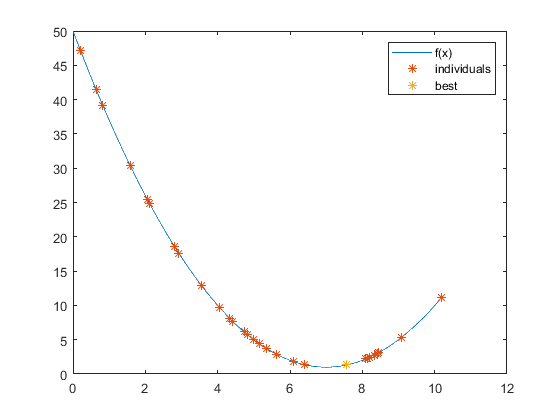
\includegraphics[width=0.5\linewidth]{Images/grafico1.png}}}%
    %\qquad
    %\hfill
    \subfloat[Ultima generazione]{{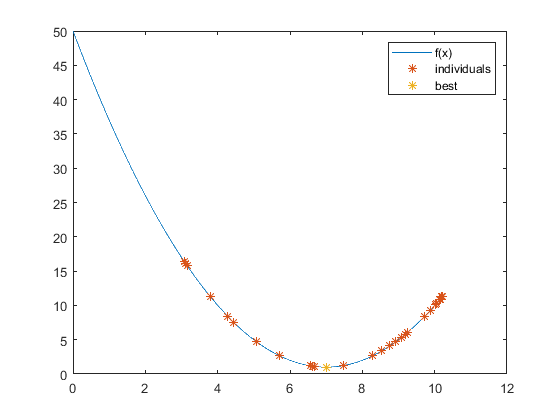
\includegraphics[width=0.5\linewidth]{Images/grafico2.png}}}%
    %\hfill
    \caption{Confronto fra la prima e l'ultima generazione del GA nel problema di minimizzazione presentato}%
    \label{fig:firstfunction}%
\end{figure}
L'immagine soprastante ci conferisce una chiara idea su come si \`e comportato il GA durante l'esecuzione: gli individui col passare delle generazioni tendono ad avvicinarsi al punto di minimo (ovvero 7 nel caso analizzato). L'algoritmo ha concluso le sue operazioni dopo poco meno di 200 iterazioni, delle quali nelle ultime 100 non si sono avuti miglioramenti di fitness, di conseguenza il ciclo \`e stato terminato forzatamente. Altre run del programma hanno portato risultati pi\`u o meno soddisfacenti per quanto concerne la distribuzione degli individui e, per via dell'esigua complessit\`a del problema, la ricerca del minimo \`e sempre terminata con successo.
\section{Considerazioni e problemi ricorrenti}
Il programma in Matlab che abbiamo presentato nell'ultima sezione pu\`o essere modificato in modo tale da minimizzare anche funzioni a due o pi\`u variabili: basterebbe soltanto modificare le funzioni di codifica e decodifica affinch\'e le stringhe che rappresentano i cromosomi contengano e restituiscano informazioni sulle variabili.

Ovviamente \`e possibile cambiare anche i parametri con cui il nostro algoritmo lavora, cos\`i da trovare quelli migliori; il tutto combinato con la possibilit\`a di cambiare anche gli operatori cardine, \`e chiaro come questo sia un indice dell'ampio margine di flessibilit\`a dei GA.
Dunque, a prima vista, il metodo da noi analizzato, ed in generale i GA, sembra essere decisamente efficiente ed efficace, ma ovviamente ad ogni pro corrisponde quasi sempre un contro.

Per mostrare il problema pi\`u ricorrente nei GA ricolleghiamoci alla sezione precedente, in particolare andiamo a testare il nostro programma con un'altra funzione, ossia $$f(x)=\cos{x}*\frac{x}{10}+2$$ sempre nell'intervallo [$0$, $10.23$]; senza riesaminare ogni funzione del nostro algoritmo nei minimi dettagli, mostriamo di seguito l'esito di una qualsiasi run.
\begin{figure}[H]%
    \centering
    %\hfill
    \subfloat[Prima generazione]{{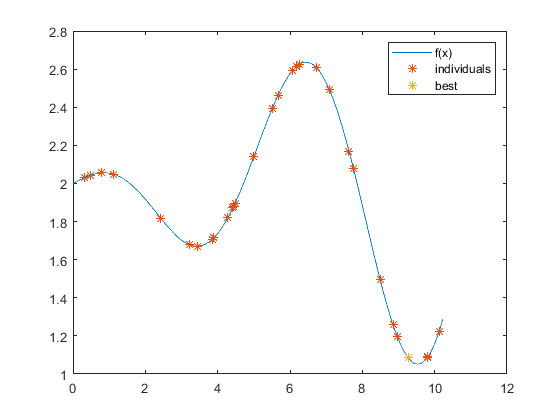
\includegraphics[width=0.5\linewidth]{Images/grafico3.png}}}%
    %\qquad
    %\hfill
    \subfloat[Ultima generazione]{{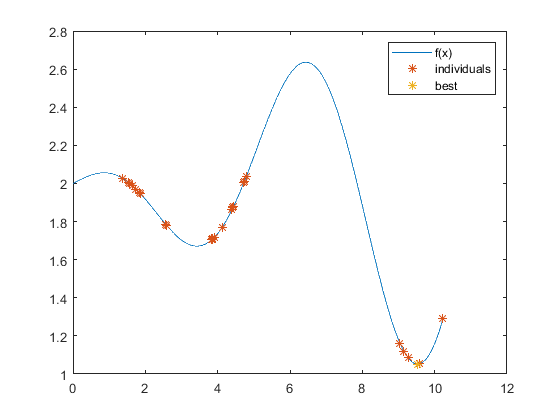
\includegraphics[width=0.5\linewidth]{Images/grafico4.png}}}%
    %\hfill
    \caption{Confronto fra la prima e l'ultima generazione per la nuova funzione considerata}%
    \label{fig:secondfunction}%
\end{figure}
Si nota subito come gli individui si siano aggregati sia nel punto di minimo assoluto (quello che noi volevamo) sia nel punto di minimo relativo, molto spesso in funzioni di questo tipo, ma anche in problemi in cui esistono "falsi ottimi", i GA possono prendere erroneamente la strada sbagliata per poi non riuscire pi\`u a ritrovare la giusta direzione (cosa che \`e successa nel nostro esempio), per ovviare a questi problemi si possono seguire diverse strategie:
\begin{itemize}
    \item Aumentare il coefficiente di mutazione, nella speranza che esso "trascini" gli individui nella direzione voluta.
    \item Ripristinare il GA come se non fosse avvenuta alcuna iterazione, soluzione drastica che non sempre porta risultati migliori di prima.
    \item Rendere "ibrido" il GA: si pensi ad un problema di ordinamento, per iniziare possiamo applicare il nostro GA, nel caso esso non veda progressi di fitness, si attua un algoritmo che sappiamo essere in grado di risolvere il problema (nel nostro caso si potrebbe usare un bubble sort per portare a termine il lavoro richiesto).
\end{itemize}

Potremmo, tramite una metafora, equiparare i GA a degli scalatori ed affermare quanto segue:
\vspace{3mm}

\begin{large}\textit{\textbf{"i GA identificano velocemente le varie vette, ma non sempre riescono a conquistare quella pi\`u alta."}}
\end{large}
\vspace{3mm}

Inoltre, per mostrare come l'approccio illustrato negli ultimi capitoli porta con s\'e alcune lacune, ci teniamo ad aggiungere ulteriori limitazioni nell'uso dei GA:
\begin{itemize}
    \item In quanto alla complessit\`a, non scalano bene all'aumentare di essa: \`e estremamente complicato usare la tecnica dei GA in problemi che possono riguardare il design di automobili o di una casa, per rendere trattabili questi problemi occorre dividerli fino alla pi\`u semplice rappresentazione possibile.
    \item Una determinata soluzione viene ritenuta come la migliore solamente rispetto alla altre, perci\`o il criterio di fermata non \`e chiaro per ogni problema.
    \item Come abbiamo fatto notare poco fa, i GA tendono a convergere verso ottimi locali e non quelli globali.
    \item Operare su insiemi di dati dinamici \`e arduo, siccome pu\`o capitare che i cromosomi convergano presto verso soluzioni non pi\`u valide per dati futuri.
    \item Non possono essere implementati efficaciemente in problemi in cui la funzione di fitness \`e data da una singola risposta booleana (come per i problemi di decisione).
    \item Nel caso vi fossero specifici problemi di ottimazzione od istanze di essi per i quali esistono tecniche risolutive ad hoc, i GA non reggono il confronto per quanto concerne la velocit\`a di convergenza verso la soluzione.
\end{itemize}
Tenendo a mente quanto affermato e mostrato finora, nei prossimi capitoli andremo ad esporre problemi pi\`u complessi rispetto a quello presentato nelle precedenti sezioni, oltre a confrontarli con altri metodi risolutivi pi\`u conosciuti.
\newpage
%\include{Chapters/colorazione_grafo}

\myChapter{Cammino minimo in un grafo}
In questo capitolo mostreremo il lavoro di un GA volto alla ricerca del cammino minimo in un grafo, a partire da un nodo v\ped{i} e terminante in un nodo v\ped{j}; l'implementazione dell'algoritmo \`e stata effettuata tramite l'uso del linguaggio Java. Nelle seguenti sezioni illustreremo il problema preso in considerazione e metteremo a confronto il GA con uno degli algoritmi pi\`u conosciuti.
\section{Descrizione del problema}
Il problema posto in esame in questo capitolo riguarda la ricerca del cammino minimo in un grafo orientato o non orientato (considereremo solo il secondo caso) da un vertice ad un altro, in modo pi\`u formale possiamo scrivere il tutto nella seguente maniera:
\vspace{3mm}

\textit{"Dato un grafo pesato (ossia un insieme di vertici V, un insieme di archi E ed una funzione f associante a ciascun arco un numero reale),  e dati due vertici distinti v\ped{i} e v\ped{j} $\in V$, trovare un cammino P=(e\ped{v\ped{i}v\ped{i+1}}, e\ped{v\ped{i+1}v\ped{i+2}}, e\ped{v\ped{i+2}v\ped{i+3}}, ..., e\ped{v\ped{j-1}v\ped{j}}) da v\ped{i} a v\ped{j} che minimizzi la somma $\sum_{e\in P} f(e)$."}
\vspace{3mm}

Sottolineamo che ogni vertice del cammino P deve essere adiacente a quello a lui precedente, ossia: preso un vertice v\ped{k} nel cammino P, fra lui e v\ped{k-1} deve esistere un arco che li connetta. Nel caso ogni arco avesse peso uguale ad 1, allora il cammino minimo risulterebbe essere quello contenente meno archi.
\vspace{3mm}

Il problema, cos\`i come lo abbiamo presentato, \`e noto anche come \textit{\textbf{problema del cammino minimo a singola coppia (single-pair shortest path problem)}}, in modo da distinguerlo dalle altre sue varianti (che non tratteremo nel corso delle successive sezioni):

\begin{itemize}
    \item \textbf{Problema del cammino minimo a singola fonte (single-source shortest path problem),} nel quale occorre trovare il cammino minimo da un singolo vertice verso tutti gli altri; sottolineiamo che ogni algoritmo risolvente tale problema, com'\`e evidente, \`e sicuramente in grado risolvere anche il single-pair shortest path problem (di fatto quest'ultimo lo rispecchia appieno, tranne nel criterio d'arresto);
    \item \textbf{Problema del cammino minimo a singola destinazione (single-destination shortest path problem),} consiste nel trovare il cammino minimo in un grafo diretto a partire da ogni vertice verso un'unica destinazione.
    \item \textbf{Problema del cammino minimo a coppie completo (all-pairs shortest path problem)}, versione amplificata di quello preso in esame in questo capitolo, infatti occorre trovare il cammino minimo fra tutte le coppie di vertici v\ped{i} e v\ped{j} nel grafo.
\end{itemize}

Dopo questa necessaria introduzione, nella prossima sezione presenteremo un algoritmo molto conosciuto, se non quello pi\`u usato ed analizzato in ambito scientifico, al fine di avere una migliore idea del problema stesso e della sua risoluzione.
\section{L'algoritmo di Dijkstra}
Una soluzione largamente apprezzata nelle ricerca del cammino minimo fu ideata da Edsger W. Dijkstra nel 1956 e pubblicata tre anni dopo, l'algoritmo ha innumerevoli varianti ma le sue forme pi\`u note riguardano il \textit{single-pair shortest path problem} (la prima in assoluto pensata da Dijkstra) ed il \textit{single-source shortest parth problem}. L'applicazione di tale algoritmo \`e vasta, in particolare \`e particolarmente apprezzata nei protocolli di routing, oltre ad essere usato come sub-routine in altri algoritmi di ricerca; ad oggi risulta essere, nella variante sviluppata da Fredman e Tarjan nel 1984, il miglior algoritmo nella risoluzione del problema che stiamo affrontando in questo capitolo.
\vspace{3mm}

L'idea dietro il funzionamento dell'algoritmo, che su parola di Dijkstra stesso fu concettualmente sviluppato in una ventina di minuti, scatur\`i dalla necessit\`a di trovare il percorso minimo per andare da una citt\`a ad un'altra; \`e immediatamente intuitivo considerare le citt\`a come vertici e le strade colleganti esse come gli archi di un grafo pesato in cui le distanze fra citt\`a corrispondono ai pesi degli archi, il tutto a patto di togliere ultieriori informazioni (semafori rossi, limiti di velocit\`a, segnali stradali ed ultieriori ostruzioni del percorso).

La facilit\`a con cui alcuni problemi si sposano con una trasformazione in un grafo, fa presto comprendere come questo approccio possa essere potente; senza ulteriori indugi illustreremo di seguito come l'algoritmo lavora.
\vspace{3mm}

Dato un vertice di partenza (noto anche come nodo inziale) in un grafo e data la \textit{distanzaY} la distanza che intercorre fra il nodo iniziale ed il nodo Y, l'algoritmo di Dijkstra assegner\`a alcuni valori iniziali di distanza e migliorer\`a in modo graduale di passo in passo la ricerca del cammino minimo:
\begin{enumerate}
    \item Impostare lo stato di tutti i nodi a "non visitato", creare al tempo stesso una lista che, di volta in volta, conterr\`a tali nodi ed un'altra lista per quelli gi\`a visitati. 
    \item Assegnare ad ogni nodo un valore di distanza iniziale, $0$ per il nodo di partenza ed un valore massimo per tutti gli altri ed inserire il nodo di partena nella lista dei "non visitati".
    \item Partendo dal nodo attuale (estratto dalla lista dei "non visitati"), calcolare la distanza \textit{provvissoria} fra tale nodo ed i suoi vicini non ancora visitati; successivamente, se la distanza \`e minore del valore assegnato al nodo su cui ci stiamo dirigendo, allora tale valore deve essere aggiornato, altrimenti non viene effettuato alcun cambio.
    \item Una volta che abbiamo terminato di considerare tutti i nodi vicini, inseriamo il nodo attuale nella lista dei "visitati".
    \item Se il nodo destinazione fosse gi\`a stato visitato, terminiamo l'esecuzione, altrimenti l'algoritmo continua fino ad aver visitato tutti i nodi (quest'ultimo approccio consente di calcolare il cammino minimo verso ogni vertice del grafo a partire dal quello designato come sorgente).
\end{enumerate}

Terminata questa doverosa premessa e spiegazione, mostriamo di seguito il codice Java relativo al funzionamento dell'algoritmo.
\definecolor{pblue}{rgb}{0.13,0.13,1}
\definecolor{pgreen}{rgb}{0,0.5,0}
\definecolor{pred}{rgb}{0.9,0,0}
\definecolor{pgrey}{rgb}{0.46,0.45,0.48}
%\usepackage{listings}
\lstdefinestyle{Java}{language=Java,
  showspaces=false,
  showtabs=false,
  numbers=left,
  frame=single,
  breaklines=true,
  showstringspaces=false,
  breakatwhitespace=true,
  commentstyle=\color{pgreen},
  keywordstyle=\color{pblue},
  stringstyle=\color{pred},
  basicstyle=\ttfamily,
  moredelim=[il][\textcolor{pgrey}]{$129$},
  moredelim=[is][\textcolor{pgrey}]{\%\%}{\%\%}
}
\begin{lstlisting}[style=Java]
public Iterator<Node> DijkstraAlgorithm(Node source, Node destination) throws Exception{
	if (!nodes.contains(source) || !nodes.contains(destination)) throw new Exception("Il nodo definito come iniziale o finale non appartiene al grafo");
		
	//Passo 1 e 2
	source.setDistance(0);
	ArrayList<Node> vNodes=new ArrayList<>();
	ArrayList<Node> nvNodes=new ArrayList<>();
	nvNodes.add(source);
		
	while (nvNodes.size()!=0) {
		Node n=minDistanceNode(nvNodes);
		nvNodes.remove(n);
		
		//siamo giunti a destinazione terminiamo, Passo 5
		if (n.equals(destination)) break;
		
		HashMap<Node, Integer> map=n.getConnectedNodes();
			
		//Passo 3
		for (Entry<Node,Integer> e: map.entrySet()) {
			Node m=e.getKey();
			
			 //necessaria per grafi non orientati
			if (vNodes.contains(m)) continue;
			
			int d=e.getValue().intValue();
			setDistance(m, n, d);
			nvNodes.add(m);
		}
			
		//Passo 4
		vNodes.add(n);
	}
	return destination.getPath();
}
\end{lstlisting}
\vspace{3mm}

Essendo l'algoritmo estremamente noto, abbiamo preso ispirazione da sue varie implementazioni circolanti nel web, in particolare la nostra versione (grazie al controllo a riga 24) permette l'uso sia per grafi orientati che non; i commenti presenti sono autoesplicativi se collegati ai 5 punti elencati prima, sottilineamo solamente i metodi \textit{minDistanceNode} e \textit{setDistance}.

Il primo permette la ricerca del nodo a minima distanza fra quelli non visitati, nel caso esso corrispondesse alla destinazione desiderata terminiamo il ciclo while (tolto questo controllo il metodo calcoler\`a i cammini minimi verso ogni nodo a partire da quello iniziale); il metodo setDistance imposta la distanza dal nodo attuale, estratto dalla lista dei "non visitati", verso un nodo ad esso connesso, nel caso la somma della distanza cumulativa del nodo attuale con il peso dell'arco collegante i due nodi sia minore della distanza cumulativa del nodo su cui vogliamo arrivare, allora aggiorneremo quest'ultimo valore ed i percorsi minimi provvisori.

Per avere una maggiore visione del codice, vi invitiamo a dare uno sguardo all'appendice a fine tesi, nella quale troverete ogni singolo sorgente usato nel corso dei vari capitoli.
%\vspace{3mm}
\section{Implementazione del GA}
Procediamo, finalmente, con l'illustrazione del codice del GA con annessa spiegazione delle varie scelte prese in sede di sviluppo del sorgente; per prima cosa, desideriamo sottolineare che l'algoritmo di Dijkstra ed il nostro algoritmo genetico appartengono alla stessa classe, ma le operazioni del GA sono definite nella classe \textit{Population.java}.

Il codice da noi sviluppato prende alcune delle idee viste in \cite{path3}, seppure apportando modifiche alle varie operazioni o eliminando quelle che abbiamo ritenuto eccessive.
\vspace{3mm}

Di seguito mostriamo la costruzione della popolazione iniziale su cui poi il GA eseguir\`a il proprio lavoro oltre alla chiamata del metodo che gestisce le sue operazioni di selezione, crossover e mutazione.
\begin{lstlisting}[style=Java]
public Chromosome ShortestPathGA(Node source, Node destination, int pSize, int maxGen, double pCrossover, double pMutation) throws Exception{
	if (nodes.size()==0) throw new Exception("Non sono stati inseriti nodi nel grafo");
	
	//Creo la popolazione e costruisco la matrice di adiacenza
	population=new Population(nodes.size(), pSize, this);
	population.buildMatrixDist(nodes.iterator());
	
	int j=0;
	while (j<pSize) {
		//Creo un cromosoma assegnandoli un percorso (geni) casuale fra sorgente e destinazione
		Chromosome c=new Chromosome(createRandomPath(source, destination));
		Iterator<Chromosome> itC=population.getChromosomes();
		
		//Controllo se tale percorso esiste gi\`a
		boolean hasSamePath=false;
		while (itC.hasNext()) {
			if (itC.next().hasSamePath(c)) {
				hasSamePath=true;
				break;
			}
		}
		if (!hasSamePath) {
			//Nel caso il cromosoma fosse unico (percorso differente dagli altri), lo aggiungo alla popolazione
			population.addChromosome(c);
			j++;
		}
	}
	
	//Eseguo il GA per un numero massimo di generazioni
	for (int i=0;i<maxGen; i++) {
		population.pathGA(pCrossover, pMutation);
	}
	return population.getFittest(); //Restituzione del miglior cromosoma
}
\end{lstlisting}
Dopo un primo controllo, il metodo provvede a creare la popolazione ed a costruire la matrice di adiacenza relativa ai nodi del grafo (tale matrice \`e usata solamente per il GA, l'algoritmo di Dijkstra non ne fa uso), successivamente costruisce cromosomi assegnando loro un percorso casuale da nodo iniziale a finale (l'idea approssima quanto espresso in \cite{path3}: un cromosoma viene aggiunto alla popolazione se e solo se il loro percorso (ovvero una sequenza di nodi corrispondente ai loro geni) risulta differente da tutti quelli gi\`a presenti nella popolazione. Questo \`e estremamente vitale per avere pi\`u diversit\`a nella popolazione, in modo da diminuire la possibilit\`a che l'algoritmo entri in stallo su soluzioni buone, ma non ottime, nelle sue prime iterazioni.

Dopo l'inizializzazione della popolazione, viene eseguito il metodo \textbf{pathGA} appartenente alla classe \textit{population} per \textit{maxGen} generazioni (numero scelto arbirtrariemente dal programmatore); il metodo termina restituendo il miglior cromosoma della popolazione finale.
\vspace{3mm}

Il metodo \textbf{pathGA} fa entrare il flusso del programma nel suo "nucleo", in quanto ha il compito di creare la nuova generazione di cromosomi a partire da quella precedente tramite i tre operatori che conosciamo gi\`a.
\begin{lstlisting}[style=Java]
public void pathGA(double pCrossover, double pMutation) {
	ArrayList<Chromosome> newGeneration=new ArrayList<>();
	while (newGeneration.size()<pSize) {
		//Selezione
		ArrayList<Chromosome> parents=selection();
		
		//Generazione di un numero casuale fra 0 ed 1
		Random r=new Random();
		double rDouble=r.nextDouble();
		
		//Crossover
		if (rDouble<pCrossover) {
			nCrossover++;
			ArrayList<ArrayList<Node>> sons=crossover(parents);
			
			//Mutazione
			mutation(sons, pMutation);
			
			//Aggiunta dei nuovi cromosomi alla popolazione
			newGeneration.add(new Chromosome(sons.get(0).iterator()));
			newGeneration.add(new Chromosome(sons.get(1).iterator()));
			
		}
	}
	newGeneration.forEach(c -> setFitness(c));
	Collections.sort(newGeneration, Chromosome.fitnessComparator);
	int i=newGeneration.size()-1;
	while (newGeneration.size()>pSize) {
		newGeneration.remove(i);
		i--;
	}
	chromosomes=newGeneration;
	best=chromosomes.get(0);
	bestFitness=best.getFitness();
}
\end{lstlisting}
Il metodo precedente rispecchia pienamente quanto detto nei capitoli passati riguardo al flusso d'esecuzione di un GA: viene creata la nuova generazione ed in seguito, fino a quando non viene raggiunta o superata la dimensione dell'attuale popolazione, vengono eseguite ripetute chiamate al metodo \textbf{selection}, il quale restituisce i due candidati genitori.

Viene, a questo punto, generato casualmente un numero reale: se esso risultasse minore del tasso di crossover, procederemo con la chiamata al metodo che si occupa di tale operazione. Dopodich\'e viene chiamato il metodo riguardante la mutazione con la successiva aggiunta dei due nuovi cromosomi alla popolazione.
%\vspace{3mm}

Al termine del ciclo principale, calcoliamo il valore di fitness (scelto come la somma delle distanze fra ogni nodo del percorso) per ogni cromosoma della nuova generazione, dopo di ci\`o riduciamo il numero di membri se necessario (potrebbe capitare con \textit{pSize} dispari di avere una generazione con dimensione maggiore di quella attuale) ed aggiorniamo i cromosomi della popolazione, calcolando al tempo stesso il migliore fra essi e la miglior fitness trovata.
\vspace{3mm}

Continuiamo l'analisi del codice sorgente con i tre metodi che implementano i tre operatori fondamentali, sui quali abbiamo gi\`a fatto abbastanza riflessioni nei capitoli precedenti: ci limiteremo ad illustrare i punti su cui differiscono da quanto visto nel capitolo 3.

Senza ulteriori premesse, presentiamo adesso il metodo relativo all'operatore di selezione.
\begin{lstlisting}[style=Java]
private ArrayList<Chromosome> selection() {
	//Dimensione del torneo
	int tSize=5;
	
	//Lista temporanea dei cromosomi
	ArrayList<Chromosome> tChroms=new ArrayList<>();
	
	chromosomes.forEach(c -> tChroms.add(c));
	Random r=new Random();
	
	//Cromosomi genitori
	ArrayList<Chromosome> parents=new ArrayList<>();
	
	while (parents.size()<2) {
		//Cromosomi partecipanti al torneo
		ArrayList<Chromosome> selChroms=new ArrayList<>();
		while (selChroms.size()<tSize) {
			int rInt=r.nextInt(tChroms.size());
			Chromosome c=tChroms.get(rInt);
			if (!selChroms.contains(c)) {
				selChroms.add(c);
			}
		}
		
		Collections.sort(selChroms, Chromosome.fitnessComparator);
		
		//Scelta del vincitore del torneo
		double p=0.75;
		double[] partialSums=new double[tSize];
		double sumP=0;
		for (int i=0;i<tSize;i++) {
			sumP+=p*Math.pow((1-p), i);
			partialSums[i]=sumP;
		}
		double rDouble=r.nextDouble()*sumP;
		int i=0;
		while (partialSums[i]<rDouble) {
			i++;
		}
		parents.add(selChroms.get(i));
		tChroms.remove(i);
	}
	return parents;
}
\end{lstlisting}
La selezione avviene nella sua variante a torneo con dimensione uguale a 5 e la scelta del miglior partecipante al torneo avviene con una probabilit\`a pari a $0.75$; successivamente il vincitore viene estratto dalla lista temporanea dei cromosomi, affinch\'e non possa essere scelto una seconda volta. Il metodo restituisce una lista contenente i due possibili genitori, i quali parteciperanno al crossover con probabilit\`a \textit{pCrossover}.
\vspace{3mm}

Parlando di crossover, \`e doveroso sottolineare che i cromosomi, come si potrebbe aver intuito, possono avere dimensioni differenti: questo causa un piccolo problema in questa fase, in quanto diventa necessario (ai fini della generazione del crossover point) calcolare la minima dimensione fra i due genitori per non incorrere in eccezioni.
\begin{lstlisting}[style=Java]
private ArrayList<ArrayList<Node>> crossover(ArrayList<Chromosome> parents) {
	//Estrazione dei due genitori dalla lista
	Chromosome parent1=parents.get(0);
	Chromosome parent2=parents.get(1);
	
	ArrayList<Node> son1=new ArrayList<>();
	ArrayList<Node> son2=new ArrayList<>();
	
	//Ottenimento dei geni dei due genitori
	Iterator<Node> itP1=parent1.getGenes();
	Iterator<Node> itP2=parent2.getGenes();
	
	//Calcolo della dimensione minima
	int minSize=parent1.getSize();
	if (parent2.getSize()<minSize) minSize=parent2.getSize();
	
	//Generazione del punto di crossover
	Random r=new Random();
	int rIndex=r.nextInt(minSize-1);
	
	//Crossover a punto singolo
	int i=0;
	while (i<rIndex) {
		son1.add(itP1.next());
		son2.add(itP2.next());
		i++;
	}
	while (itP1.hasNext()) {
		son2.add(itP1.next());
	}
	while (itP2.hasNext()) {
		son1.add(itP2.next());
	}
	
	//Restituzione dei due figli
	ArrayList<ArrayList<Node>> sons=new ArrayList<>();
	sons.add(son1);
	sons.add(son2);
	return sons;
}
\end{lstlisting}
A differenza di quanto fatto da \cite{path3} (in cui il crossover point viene scelto fra geni identici dei due cromosomi), generiamo il punto di crossover \textit{rIndex} nell'intervallo [0, minSize-1], i tre while eseguono lo stesso lavoro di un crossover a punto singolo che abbiamo potuto osservare nel capitolo 3; il metodo termina restituendo una lista di percorsi e non i due cromosomi: questa soluzione \`e scelta in modo che la mutazione avvenga prima dell'effettiva creazione dei due oggetti relativi ai figli, modificare direttamente un array \`e molto pi\`u semplice che lavorare con iteratori per poi aggiornare i geni dell'individuo.
\vspace{3mm}

Terminiamo la sezione con il metodo riguardante la mutazione, niente di nuovo rispetto a quanto visto nei capitoli precedenti se non per una modifica che risulta fondamentale per la riuscita dell'algoritmo in s\'e.
\begin{lstlisting}[style=Java]
private void mutation(ArrayList<ArrayList<Node>> individuals, double pMutation) {
	Random r=new Random();
	for (int i=0;i<individuals.size();i++) {
		ArrayList<Node> son=individuals.get(i);
		for (int j=0;j<son.size()-1;j++) {
			double rDouble=r.nextDouble();
			
			//Se la mutazione avviene, trovo un nuovo percorso dal nodo scelto verso la destinazione
			if (rDouble<pMutation) {
				nMutation++;
				Node n=son.get(j);
				Node d=son.get(son.size()-1);
				Iterator<Node> itN= graph.createRandomPath(n, d);
				
				//Eliminimo gli elementi successivi al nodo che ha subito la mutazione
				for (int k=son.size()-1;k>=j;k--) {
					son.remove(k);
				}
				
				//Aggiungo il percorso
				while (itN.hasNext()) son.add(itN.next());
				break;
			}
		}
		
		//Elimino i nodi dupilcati
		son=(ArrayList<Node>)son.stream().distinct(). collect(Collectors.toList());
	}
}
\end{lstlisting}
La mutazione, che agisce unicamente su un gene, crea un percorso casuale (con lo stesso metodo \textbf{createRandomPath} dell classe Graph) a partire dal gene stesso fino alla destinazione; in seguito elimina i geni successivi a quello da cui abbiamo calcolato il percorso ed aggiorna quello totale, eliminando inoltre i potenziali geni duplicati creatisi con il crossover e/o con la mutazione.
\vspace{3mm}

L'algoritmo, come si pu\`o notare dai codici esaminati, fa uso di altri metodi di supporto non inseriti in questa sezione: come sempre, saranno disponibili al termine della tesi nell'apposita appendice. L'obiettivo che rimane adesso \`e mostrare l'efficacia effettiva del nostro approccio.
\section{Analisi di un esempio}
In questa sezione porremo sotto esame il comportamento del nostro GA appena descritto, ma prima occorre senza dubbio avere a disposizione un grafo su cui operare. Grazie ad un tool online trovato su graphonline.ru e alla costruzione degli oggetti relativi ai nodi ed agli archi in Java, siamo riusciti a creare un grafo non orientato con $20$ vertici numerati da $0$ a $19$, dopodich\'e abbiamo inserito i dati nel nostro programma (nodo iniziale e nodo finale) ed abbiamo applicato l'algoritmo di Dijkstra.
\begin{figure}[H]
    \centering
    \hfill
    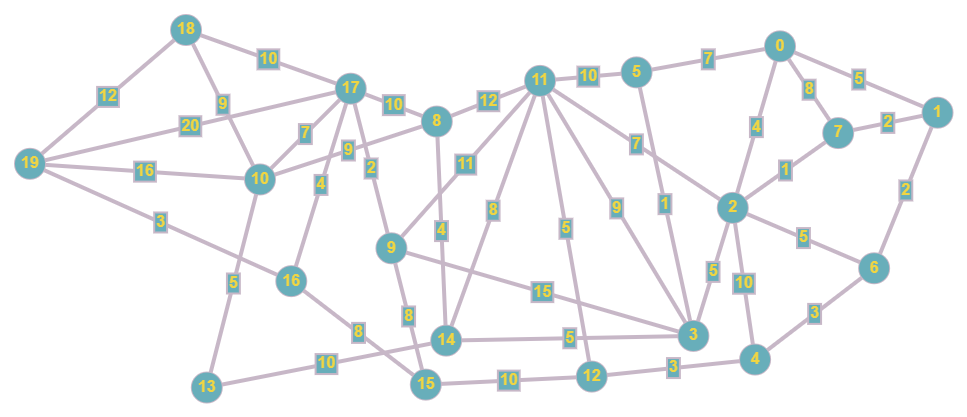
\includegraphics[width=1\textwidth]{Images/graph.png}
    \hspace*{\fill}
    \caption{Il grafo preso in esame}
    \label{fig:graph}
\end{figure}
Il nostro obiettivo consisteva nel trovare in tale grafo il cammino minimo da un nodo iniziale ad uno finale: per tutta la sezione supporremo di dover partire dal nodo $0$ e terminare nel nodo $19$; tale cammino sar\`a vitale nell'analisi del funzionamento del GA.
\vspace{3mm}

Per testare il funziomento dell'algoritmo di Dijkstra da noi implementato lo abbiamo messo a confronto con un calcolatore online: i risultati sono stati tutti positivi, dunque per testare il lavoro del nostro GA ci siamo basati sulle risposte dell'algoritmo di Dijkstra costruito nella nostra classe Graph.

Come detto poco fa, il nostro scopo era calcolare il minimo cammino dal nodo $0$ al nodo $19$, nell'immagine sottostante si pu\`o osservare da quali nodi sia formato.
\begin{figure}[H]
    \centering
    \hfill
    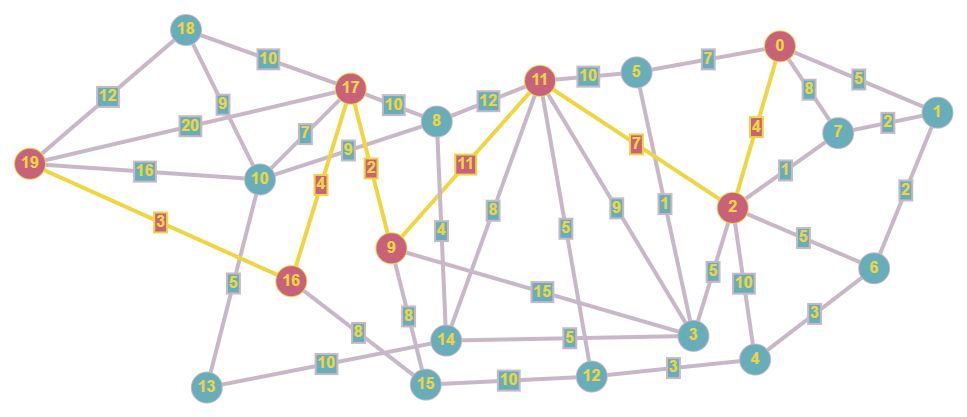
\includegraphics[width=1\textwidth]{Images/path.png}
    \hspace*{\fill}
    \caption{Il cammino minimo calcolato dall'algoritmo di Dijkstra}
    \label{fig:path}
\end{figure}
Il cammino risulta avere una lunghezza pari a 31, questo ci permette di avere un valore di riferimento utile per mostrare ed analizzare i risultati scaturiti dal lavoro del GA.
\vspace{3mm}

L'algoritmo genetico ha dato risultati molto eterogenei fra di loro a seconda dei parametri inseriti, in ogni caso precisiamo che i nosti valori di partenza corrispondono a:
\begin{itemize}
    \item Numero massimo di iterazioni (\textit{maxIt}), $30$;
    \item Dimensione della popolazione (\textit{pSize}), $40$;
    \item Tasso di mutazione, $0.1$;
    \item Tasso di crossover, $0.90$
    \item Dimensione del torneo (\textit{tSize}), $5$;
    \item Tasso di scelta del migliore del torneo, $0.75$;
\end{itemize}
%aver mai alterato il numero massimo di iterazioni ($30$), la dimensione del torneo di selezione ($5$) e la relativa probabilit\`a di scelta del vincitore ($0.75$).
Nella nostra analisi abbiamo agito sui primi cinque parametri, ma non abbiamo rilevato enormi differenze agendo sui tassi di mutazione e crossover (i migliori risultati sono stati ottenuti con i valori specificati e che rimarrano gli stessi per tutta l'analisi), di conseguenza sono stati la dimensione della popolazione  e del torneo uniti al numero massimo di iterazioni ad aver determinato maggiormente l'efficacia del nostro algoritmo.
%abbiamo agito sulla dimensione della popolazione, sulla dimensione del torneo di selezione, sul numero massimmo di iterazioni, sul crossover e sulla mutazione; ma sono state sicuramente le prime $3$ ad aver avuto il maggior impatto rispetto alle altre due.
\vspace{3mm}

Per ogni valore di \textit{pSize} (dimensione della popolazione, lasciando immutati tutti gli altri) nell'intervallo [$10$, $50$], con passo uguale a $5$ (valori di pSize<=$5$ collidono con la dimensione del torneo), abbiamo eseguito 200 run, calcolando per ognuna di esse: la fitness del miglior cromosoma trovato, la fitness del peggior cromosoma trovato (ma pur sempre il migliore della sua run) e la fitness media. Dal grafo si pu\`o notare come l'unico percorso minimo con lunghezza $31$ dal nodo iniziale a quello finale sia $$0 -> 2 -> 11 -> 9 -> 17 -> 16-> 19$$ perci\`o ogni volta che troveremo un cammino di lunghezza $31$ possiamo essere certi che sia lui (aggiungiamo che lanciando singole run, il cammino ottenuto dal GA coincide perfettamente).
\begin{center}
\begin{table}[H]
    \centering
    \begin{tabular}{|C{2cm}C{3.25cm}C{3.25cm}C{3.25cm}|}
        \hline
        \textbf{pSize}  & \textbf{Best Fitness} & \textbf{Worst Fitness} & \textbf{Average Fitness} \\ \hline
        
        \cellcolor{mygray!35} $10$ & \cellcolor{mygray!35} $31$ & \cellcolor{mygray!35} $91$ & \cellcolor{mygray!35} $42.055$ \\
        
        $15$ & $31$ & $66$ & $36.905$ \\
        
        \cellcolor{mygray!35} $20$ & \cellcolor{mygray!35} $31$ & \cellcolor{mygray!35} $63$ & \cellcolor{mygray!35} $36.825$ \\ 
        
        $25$ & $31$ & $59$ & $34.97$ \\
        
        \cellcolor{mygray!35} $30$ & \cellcolor{mygray!35} $31$ & \cellcolor{mygray!35} $52$ & \cellcolor{mygray!35} $34.35$ \\
        
        $35$ & $31$ & $48$ & $34.48$ \\
        
        \cellcolor{mygray!35} $40$ & \cellcolor{mygray!35} $31$ & \cellcolor{mygray!35} $45$ & \cellcolor{mygray!35} $33.71$ \\
        
        $45$ & $31$ & $42$ & $33.135$ \\
        
        \cellcolor{mygray!35} $50$ & \cellcolor{mygray!35} $31$ & \cellcolor{mygray!35} $41$ & \cellcolor{mygray!35} $33.07$ \\
        
        %50 & ND & ND & ND \\
        
        %\cellcolor{mygray!35} 50 & \cellcolor{mygray!35} ND & %\cellcolor{mygray!35} ND & \cellcolor{mygray!35} ND \\
        
        \hline
        
        \textbf{Averages} & $31$ & $56.33$ & $35.5$ \\
        
        \hline
    \end{tabular}
    \caption{Risultati ottenuti con 200 run a valori differenti di pSize}
    \label{tab:table1}
\end{table}
\end{center}
Come possiamo notare dalla tabella soprastante, a valori fissi degli altri parametri, si vede chiaramente come una popolazione maggiore apporti benefici al calcolo del cammino minimo, ma al tempo stesso comporta un maggior tempo di esecuzione del programma, unito al fatto che per valori di pSize estremamente elevati l'algoritmo entra in loop dato che (per come abbiamo impostato il setup della popolazione) non riesce a generare abbastanza percorsi casuali in modo da costruire la prima generazione di cromosomi.
Inoltre, a giudicare dalla fitness media, pare che la miglior scelta della dimensione della popolazione risulti essere per valori superiori a $20$, ma questo non ci dice tutto quello che desideriamo.
\vspace{3mm}

Infatti la tabella assume maggiore significato se includiamo anche il tasso di successo del GA a valori di \textit{pSize} differenti, ovvero la percentuale con cui il nostro algoritmo su $200$ run \`e riuscito a trovare il cammino minimo, il tutto confrontato col tempo di esecuzione, parametro di cui ancora non abbiamo tenuto conto.

Invitiamo a leggere la successiva tabella contenente le informazioni menzionate poco fa nello stesso paragrafo.
\begin{center}
    \begin{table}[H]
        \centering
        \begin{tabular}{|C{3cm}C{3cm}C{5.75cm}|}
            \hline
            \textbf{pSize} & \textbf{\%Success} & \textbf{Execution Time (200 run)} \\ \hline
            
            \cellcolor{mygray!35} $10$ & \cellcolor{mygray!35} $3.5\%$ & \cellcolor{mygray!35} $386ms$ \\
            
            $15$ & $8\%$ & $426ms$ \\
            
            \cellcolor{mygray!35} $20$ & \cellcolor{mygray!35} $9.5\%$ & \cellcolor{mygray!35} $501ms$ \\
            
            $25$ & $11.5\%$ & $615ms$\\
            
            \cellcolor{mygray!35} $30$ & \cellcolor{mygray!35} $15.5\%$ & \cellcolor{mygray!35} $707ms$ \\
            
            $35$ & $18\%$ & $904ms$ \\
            
            \cellcolor{mygray!35} $40$ & \cellcolor{mygray!35} $21.5\%$ & \cellcolor{mygray!35} $978ms$\\
            
            $45$ & $25\%$ & $1109ms$ \\
            
            \cellcolor{mygray!35} $50$ & \cellcolor{mygray!35} $28\%$ & \cellcolor{mygray!35} $1241ms$ \\
            
            \hline
        
            \textbf{Averages} & $15.61\%$ & $763ms$ \\
            
            \hline
            
        \end{tabular}
        \caption{Tassi di successo su 200 run con valori di pSize nell'intervallo [$10$, $50$]}
        \label{tab:table2}
    \end{table}
\end{center}
Osservando attentamente le due tabelle, possiamo stabilire che i valori di \textit{pSize} migliori risultano nell'intervallo [$40$, $50$], dobbiamo sottolineare per\`o che il miglior valore di successo che abbiamo ottenuto \`e solo del $28\%$, valore che non ci concede buone speranze nell'affidarci al GA.
\vspace{3mm}

Un aspetto molto importante viene assunto, a questo punto, dalla selezione: come abbiamo detto abbiamo implementato tale operatore nella sua versione a torneo e la dimensione di quest'ultimo, se non impostata attentamente, rischia di causare gravi danni alla ricerca del cammino minimo. Di fatto la selezione a torneo \`e stata ampiamente analizzata e discussa da \cite{selection1} e \cite{selection2}, noi ci limiteremo a mostrare (tramite la tabella di seguito) come essa possa influire sul nostro algoritmo; facciamo notare, inoltre, che non abbiamo inserito i valori per \textit{tSize} uguale ad $1$ (come detto nel capitolo $2$, sarebbe puramente una selezione casuale) e per valori di \textit{tSize}>=$5$ non abbiamo riscontrato sostanziali differenze (ci siamo limitati a riportare i valori della precedente tabella, i dati di essa erano stati ottenuti proprio con tSize uguale a $5$).
\begin{center}
    \begin{table}[H]
        \centering
        \begin{tabular}{|C{2.15cm}C{2.15cm}C{2.15cm}C{2.15cm}C{2.15cm}|}
            \hline
            & \multicolumn{4}{C{8.60cm}|}{\textbf{\%Success}} \\ \cline{2-5}
            \textbf{pSize} & \textbf{tSize==2} & \textbf{tSize==3} & \textbf{tSize==4} & \textbf{tSize>=5} \\ \hline
            
            \cellcolor{mygray!35} $10$ & \cellcolor{mygray!35} $0\%$ & \cellcolor{mygray!35} $0.5\%$ & \cellcolor{mygray!35} $2\%$ & \cellcolor{mygray!35} $3.5\%$ \\
            
            $15$ & $0\%$ & $0.5\%$ & $6\%$ & $8\%$ \\
            
            \cellcolor{mygray!35} $20$ & \cellcolor{mygray!35} $0.5\%$ & \cellcolor{mygray!35} $0\%$ & \cellcolor{mygray!35} $6\%$ & \cellcolor{mygray!35} $9.5\%$ \\
            
            $25$ & $0\%$ & $2\%$ & $2.5\%$ & $11.5\%$ \\
            
            \cellcolor{mygray!35} $30$ & \cellcolor{mygray!35} $0\%$ & \cellcolor{mygray!35} $1.5\%$ & \cellcolor{mygray!35} $9.5\%$ & \cellcolor{mygray!35} $15.5\%$ \\
            
            $35$ & $2\%$ & $0.5\%$ & $10\%$ & $18\%$ \\
            
            \cellcolor{mygray!35} $40$ & \cellcolor{mygray!35} $0\%$ & \cellcolor{mygray!35} $1.5\%$ & \cellcolor{mygray!35} $13.5\%$ & \cellcolor{mygray!35} $21.5\%$ \\
            
            $45$ & $1\%$ & $2.5\%$ & $14.5\%$ & $25\%$ \\
            
            \cellcolor{mygray!35} $50$ & \cellcolor{mygray!35} $2\%$ & \cellcolor{mygray!35} $3\%$ & \cellcolor{mygray!35} $18.5\%$ & \cellcolor{mygray!35} $28\%$ \\
            
            \hline
        
            \textbf{Averages} & $0.61\%$ & $1.44\%$ & $9.16\%$ & $15,61\%$ \\
            
            \hline
            
        \end{tabular}
        \caption{Tassi di successo su 200 run con valori di pSize nell'intervallo [$10$, $50$] e a valori differenti di tSize}
        \label{tab:table3}
    \end{table}
\end{center}
\vspace{3mm}
Come la tabella ci mostra, valori di \textit{tSize} troppo piccoli, nel caso in esame, non risultano affidabili e quelli oltre il valore 5 causano un aumento del tempo di esecuzione senza aumenti notevoli del tasso di successo.

I valori ottenuti a questo punto ci fanno capire che una buona scelta d'implementazione della selezione, specialmente se a torneo, consente di aumentare notevolmente l'efficacia del nostro algoritmo.
\vspace{3mm}

A questo punto non ci rimane altro che illustrare come il numero di iterazioni influisce sull'efficacia del nostro approccio, la tabella di seguito mostra i tassi di successo ricavati al cambio di \textit{maxIt} e di \textit{pSize}, lasciando invariati tutti gli altri.
\begin{center}
\begin{table}[H]
    \centering
    \begin{tabular}{|C{2.18cm}C{2.18cm}C{2.18cm}C{2.18cm}C{2.18cm}C{2.18cm}|}
        \hline
        \textbf{pSize} & \textbf{maxIt=30} & \textbf{maxIt=60} & \textbf{maxIt=90} & \textbf{maxIt=120} \\ \hline
        
        \cellcolor{mygray!35} $10$ & \cellcolor{mygray!35} $3.5\%$ & \cellcolor{mygray!35} $6\%$ & \cellcolor{mygray!35} $6\%$ & \cellcolor{mygray!35} $7\%$ \\
            
        $15$ & $8\%$ & $11.5\%$ & $18.5\%$ & $21.5\%$ \\
            
        \cellcolor{mygray!35} $20$ & \cellcolor{mygray!35} $9.5\%$ & \cellcolor{mygray!35} $14.5\%$ & \cellcolor{mygray!35} $22.5\%$ & \cellcolor{mygray!35} $25\%$ \\
            
        $25$ & $11.5\%$ & $22\%$ & $29\%$ & $33.5\%$ \\
            
        \cellcolor{mygray!35} $30$ & \cellcolor{mygray!35} $15.5\%$ & \cellcolor{mygray!35} $22\%$ & \cellcolor{mygray!35} $33\%$ & \cellcolor{mygray!35} $36\%$ \\
            
        $35$ & $18\%$ & $26.5\%$ & $34.5\%$ & $40.5\%$ \\
            
        \cellcolor{mygray!35} $40$ & \cellcolor{mygray!35} $21.5\%$ & \cellcolor{mygray!35} $28\%$ & \cellcolor{mygray!35} $41.5\%$ & \cellcolor{mygray!35} $45\%$ \\
            
        $45$ & $25\%$ & $31.5\%$ & $43\%$ & $50.5\%$ \\
            
        \cellcolor{mygray!35} $50$ & \cellcolor{mygray!35} $28\%$ & \cellcolor{mygray!35} $38.5\%$ & \cellcolor{mygray!35} $50\%$ & \cellcolor{mygray!35} $56\%$ \\
            
        \hline
        
        \textbf{Averages} & $15.61\%$ & $22.77\%$ & $30.88\%$ & $35\%$ \\
        
        \hline
    \end{tabular}
    \caption{Tassi di successo su 200 run con valori di pSize in [$10$, $50$], a valori differenti di maxIt}
    \label{tab:table4}
\end{table}
\end{center}
Come possiamo notare il numero di iterazioni agisce in modo pi\`u decisivo rispetto agli altri parametri, ma al tempo stesso il suo tempo di esecuzione aumenta esponenzialmente, per ovviare a questo si potrebbe terminare l'esecuzione dell'algoritmo dopo un numero arbitrario di cicli di esecuzione (per esempio se la fitness non migliora per un terzo delle iterazioni complessive), in modo da diminuire il suo tempo di runtime.

Vogliamo precisare, per\`o, che i valori ottenuti durante questa sezione possono essere migliorati ancora attuando opportune modifiche agli altri valori che nella nostra analisi non abbiamo toccato (per esempio il tasso di crossover o mutazione, per citarne alcuni), oppure aggiungendo un tasso di elitismo, cosa che permetterebbe la sopravvivenza dei cromosomi migliori di generazione in generazione.
%sicuramente il parametro che influisce maggiormente fra quelli rimasti corrisponde al numero di iterazioni massime.
%Quest'ultimo, che nelle tabelle precedenti era fissato a 30, rappresenta una scelta implementativa di immenso impatto ai fini della ricerca, la seguente tabella mostra chiaramente come influisca (gli altri valori, tranne pSize, rimangono sempre quelli definiti inzialmente).
%\begin
Nella prossima sezione, porremo in evidenza le migliorie applicabili al nostro approccio unite a considerazioni sorte durante lo sviluppo e la gestione dell'algoritmo.
\section{Conclusioni sul lavoro del GA}
Con molta probabilit\`a l'esito mostrato nella sezione precedente lascerebbe molto a desiderare sulla possibilit\`a di un impiego dei GA per tale problema: in effetti, soprattutto per grafi con numero esiguo di vertici, l'algoritmo di Dijkstra risulta migliore sotto ogni punto di vista, ma questo non ci deve assolutamente limitare.

Infatti, come abbiamo gi\`a detto, abbiamo illustrato solamente come alcuni indicatori cambiano al variare della dimensione della popolazione, non abbiamo tenuto conto che ci sono molti altri parametri su cui non abbiamo influito (basta pensare al numero massimo di iterazioni o al tasso di mutazione), oltre al fatto che anche il calcolo della fitness non sia il migliore in assoluto: persino nel capitolo 3 abbiamo sottolineato come una buona funzione di fitness possa stravolgere completamente l'andamento di un GA.
\vspace{3mm}

Laddove noi abbiamo semplicemente usato la somma dei costi degli archi fra nodi adiacenti che fanno parte del cammino, ricercatori del settore hanno utilizzato una funzione decisamente migliore, la quale risulta essere \cite{path2} : $$f(x)=\frac{1}{path\_length}-\#disconnected\_nodes$$ dove \textit{path\_length} corrisponde alla lunghezza del cammino e \#disconnected\_nodes \`e un intero che assume valore $0$ od $1$ (quest'ultimo se e solo se vi sono nodi consecutivi non adiacenti nel cammino).
La prossima ed ultima tabella illustra come questa funzione di fitness possa migliorare il nostro approccio (i cambiamenti eseguiti per implementare la nuova funzione di fitness non sono stati ingenti, per questo motivo non sono stati inseriti in appendice). Per correttezza, sottolineiamo che i parametri non inseriti esplicitamente in tabella risultano essere uguali a quanto visto ad inzio sezione.
\begin{center}
    \begin{table}[H]
        \centering
        \begin{tabular}{|C{3.95cm}C{3.95cm}C{3.95cm}|}
            \hline
            \textbf{maxIt} & \textbf{Nostra f(x)} &\textbf{Nuova f(x)\cite{path2}} \\ \hline
            
            \cellcolor{mygray!35} $30$ & \cellcolor{mygray!35} $21.5\%$ & \cellcolor{mygray!35} $25.5\%$ \\
            
            $60$ & $28\%$ & $35\%$ \\
            
            \cellcolor{mygray!35} $90$ & \cellcolor{mygray!35} $41.5\%$ & \cellcolor{mygray!35} $42\%$ \\
            
            $120$ & $45\%$ & $49\%$ \\
            
            \cellcolor{mygray!35} $150$ & \cellcolor{mygray!35} $50.5\%$ & \cellcolor{mygray!35} $51.5\%$ \\
            
            \hline
            
            \textbf{Averages} & $37.3\%$ & $40.6\%$ \\
            
            \hline
        \end{tabular}
        \caption{Tassi di successo su 200 run per funzioni differenti al cambiare del numero massimo di iterazioni}
        \label{tab:table5}
    \end{table}
\end{center}
La nuova funzione proposta non apporta grandi cambiamenti nei tassi di successo, per la maggior parte dovuto al fatto che la nostra implementazione non si sposa perfettamente con la soluzione proposta da \cite{path2}, avremmo dovuto agire maggiormente sulla creazione della prima generazione e sul crossover (per esempio impostare il \textit{crossover-point} in un nodo comune ai due cromosomi genitori).
\vspace{3mm}

Aggiungiamo inoltre che, nella grande maggioranza dei casi, viene sempre tenuto in considerazione un determinato valore di elitismo (solitamente fra il $5\%$ ed il $30\%$), ma quest'ultimo potrebbe rivelarsi un'arma a doppio taglio: sappiamo infatti che i GA possono cadere in \textit{falsi ottimi} e non riuscire a trovare una giusta alternativa fra le soluzioni generate.
Nel nostro esempio, abbiamo effettuato qualche test con valori di elitismo dallo $0\%$ al $50\%$, ottenendo scarsi ed irrilevanti miglioramenti sui tassi di successo del nostro algoritmo: l'applicazione dell'elitismo non risulta una scelta obbligatoria per ogni dato problema.
\vspace{3mm}

Altre soluzioni migliori proposte nel corso degli anni hanno proposto algoritmi genetici ibridi \cite{path1}, oppure di partire con valori di selezione molto alti e di mutazione molto bassi \cite{path5}, per poi cambiarli dinamicamente nel corso dell'esecuzione.

Come abbiamo evidenziato nei capitoli precedenti, i GA non reggono il confronto contro algoritmi ad hoc per la soluzione di determinati problemi (come lo era l'algoritmo di Dijkstra nel caso in esame), ma, rimanendo nell'ambito del cammino minimo, possono avere voce in capitolo in quei problemi dove \`e preferibile avere una soluzione ritenuta \textit{buona} in tempi ragionevoli, a discapito della ricerca dell'ottimo: l'esempio pi\`u conosciuto riguarda il routing dei dati in una rete.

Possiamo quindi affermare senza alcun dubbio che:
\vspace{3mm}

\begin{large}\textit{\textbf{"la buona implementazione e, di conseguenza, l'efficacia di un GA dipendono dalle capacit\`a decisionali, dalla resilienza e dalla flessibilit\`a d'ingegno del programmatore."}}
\end{large}
\vspace{3mm}

Con questo vi lasciamo al prossimo capitolo, nel quale discuteremo di altri problemi basati sui grafi risolvibili (o almeno che siano in grado di dare una soluzione buona) tramite l'uso dei GA, per poi dare una conclusione a quanto visto in questa tesi portando altri vari ambiti di applicazione dell'approccio che ci ha accompagnato per tutti i capitoli e delle riflessioni rapide sul suo futuro.
%uno di questi esempi conterr\`a un utilizzo su un noto gioco che si sposa perfettamente con l'uso dei grafi.
%Con questo vi lasciamo alle conclusioni riguardanti i GA, tratte durante tutto l'arco del tirocinio e che avranno spazio nel prossimo ed ultimo capitolo di questa tesi.
\newpage

\myChapter{Ulteriori applicazioni e conclusioni}
In quest'ultimo capitolo elencheremo ulteriori possibili campi di applicazione dei GA, ricongiugendoci con quanto visto nella risoluzione del problema del cammino minimo, per poi rimanere, successivamente, nell'ambito di casi di studio relativi ai grafi, terminando con una visione generale sugli sviluppi attuali e futuri dei GA, consci di quanto osservato durante la tesi.
%\section{Ulteriori applicazioni sui grafi}

Sebbene il precedente capitolo vertesse solamente sull'implemetanzione, non ottimale, di un GA nella risoluzione del problema del cammino minimo, durante il tirocinio sono stati presi in considerazione molteplici casi di studio riguardo ai grafi; in particolare la nostra attenzione si \`e soffermata principalmente su due problemi molto conosciuti nel mondo scientifico: il problema del commesso viaggiatore \cite{tsp1} (Travelling Salesman Problem, TSP, di cui parleremo molto rapidamente) e della colorazione di un grafo\cite{graphcol6}.
\section{Il problema del commesso viaggiatore}
Per chi \`e esperto del settore questo problema sar\`a ben noto, ma comunque descriveremo velocemente in cosa consiste citando la domanda che esso pone:
\vspace{3mm}

\textit{Data una lista di citt\`a e date le distanze fra coppie di esse, qual \`e il cammino minimo possibile che attraversa tutte le citt\`a e che termina in quella di partenza?}
\vspace{3mm}
\begin{figure}[H]%
    \centering
    %\hfill
    \subfloat[Insieme di citt\`a]{{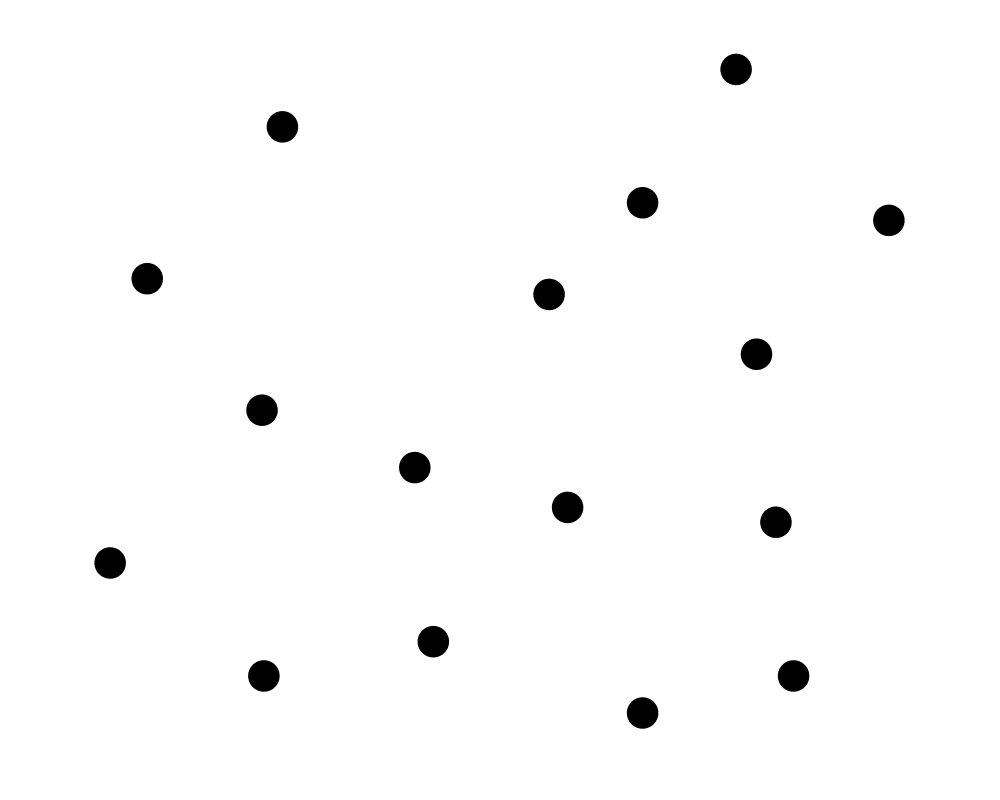
\includegraphics[width=0.5\linewidth]{Images/tspStart.png}}}%
    %\qquad
    %\hfill
    \subfloat[Una possibile soluzione]{{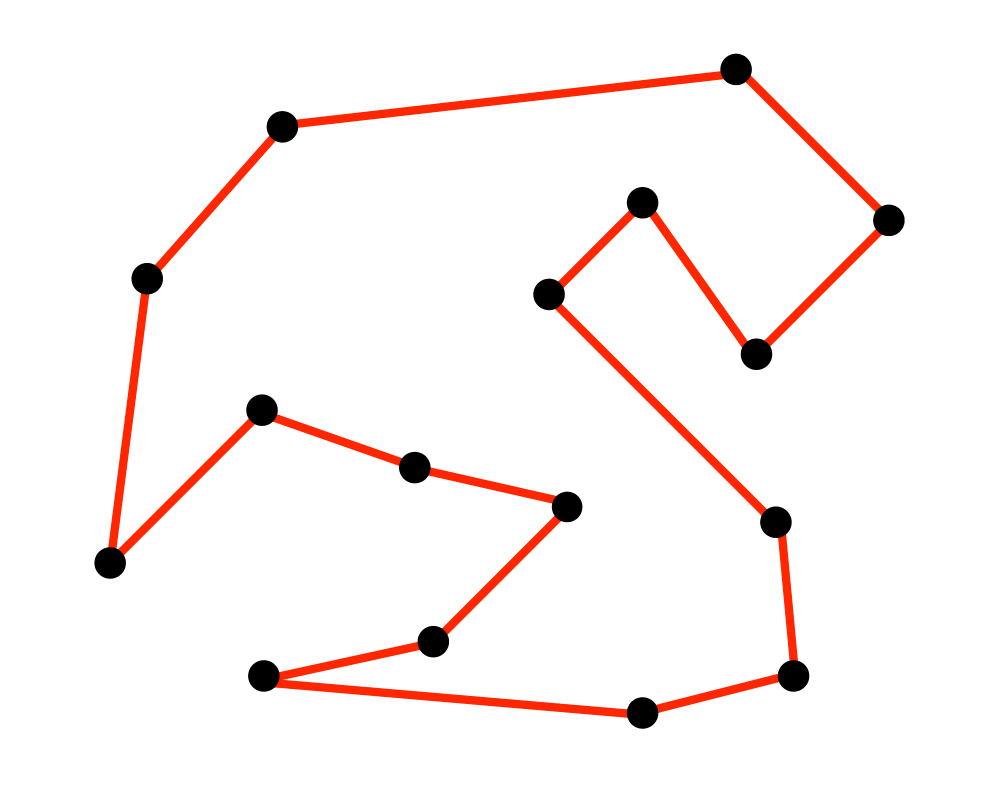
\includegraphics[width=0.5\linewidth]{Images/tspEnd.png}}}%
    %\hfill
    %\caption{Confronto fra la prima e l'ultima generazione per la nuova funzione considerata}%
    \caption{Il problema del commesso viaggiatore, fonte: algorist.com}
    \label{fig:tsp}%
\end{figure}
A prima vista la domanda posta dal problema potrebbe risultare simile a quella vista all'inizio del capitolo 5, la differenza consiste nel fatto che essa richieda il calcolo del migliore \textit{ciclo hamiltoniano} che un possibile commesso possa intraprendere fra tutte le citt\`a.

La maggiore difficolt\`a risiede, per determinare l'efficacia di un possibile GA, nel fatto che mancano algoritmi efficienti per la risoluzione nel caso di un'ingente quantit\`a di citt\`a, lasciandoci senza valori di riferimento come lo era stato l'algoritmo di Dijkstra nel capitolo precedente; il problema, che viene usato anche come standard di valutazione per numerosi algoritmi di ricerca, \`e di una complessit\`a computazionale elevata (pari ad O(n!) per algoritmi esatti, con n numero di citt\`a e considerato il caso peggiore in cui ogni nodo risulta connesso a tutti gli altri), di fatto \`e stato possibile risolvere il problema con precisione fino ad una decina di migliaia di citt\`a, ottenendo non grandi margini di errori per un'insieme di milioni di citt\`a.
\vspace{3mm}

Come per la ricerca del cammino minimo, anche il TSP, a sua volta in maniera simile, pu\`o essere espresso come un problema basato sui grafi: le citt\`a corrisponderebbero ai vertici, le congiunzioni fra le citt\`a risultano gli archi e le distanze come i pesi di tali archi; il tutto, dunque, si trasforma in un problema di minimizzazione che parte e termina in uno stesso vertice, effettuando la visita una ed una sola volta di ogni altro vertice in un grafo non orientato e pesato.
\vspace{3mm}

Seppur paradossale, l'approccio con i GA risulta, secondo \cite{path4}, di pi\`u semplice implementazione rispetto al calcolo del cammino minimo: i cromosomi rappresentanti i vari cicli, avrebbero tutti la stessa lunghezza e sappiamo come la gestione di lunghezze differenti causi maggiore complessit\`a in fase di implementazione (abbiamo avuto la possibilit\`a di sperimentare sulla nostra pelle questo fatto).
\vspace{3mm}

I tentativi di dare una soluzione al problema tramite l'uso dei GA sono stati molti, in particolare Heinrich Braun \cite{tsp2} \`e stato in grado (migliorando quanto fatto da Muhlenbein e colleghi \cite{tsp3}) di trovare una soluzione ottimale fino a 442 citt\`a; inoltre sono stati effettuati diversi studi su quanto le scelte di implementazione effettuate sui vari operatori \cite{tsp5} (che ricordiamo per l'ennesima volta essere: selezione, crossover e mutazione) influiscono sull'efficacia nel trovare il ciclo minimo, in particolare una buona scelta fra le possibili varianti della selezione permette, come dimostrato da \cite{tsp4}, di ottenere risultati migliori.
\vspace{3mm}

Avendo trattato fino ad ora due dei maggiori problemi di minimizzazione incentrati su cammini e cicli minimi, passeremo nella prossima sezione ad osservare un altro ambito di applicazione dei GA sempre relativo ad un problema riguardante i grafi.
%Inoltre, sempre riguardo gli operatori nel contesto del TSP, 
%\begin{center}
%\begin{table}[]
    %\centering
%    \begin{tabular}{C|C|C|C|C}
    %     &  \\
     %    & 
 %   \end{tabular}
%    \caption{Caption}
%    \label{tab:my_label}
%\end{table}
%\end{center}
\section{Colorazione di un grafo}
La colorazione di un grafo consiste, come il nome ci suggerisce, nell'assegnare ad ogni vertice di un grafo un colore (od etichetta) in modo tale che nessun vertice condivida la stessa etichetta con quelli a lui adiacenti, pi\`u nel dettaglio il problema pu\`o essere espresso come:
\vspace{3mm}

\textit{Dato un grafo G, calcolare il \textit{numero cromatico} $\chi(G)$, ovvero trovare il numero minimo di colori necessari affinch\'e nessun nodo condivida un colore con quelli a s\'e adiacenti.}
\vspace{3mm}

Casi analoghi riguardano la colorazione delle facce di un grafo planare o degli archi, ma in questa sezione discuteremo solamente della colorazione dei vertici e della nostra semplice implementazione in Java.
\vspace{3mm}
\begin{figure}[H]
    \centering
    \hfill
    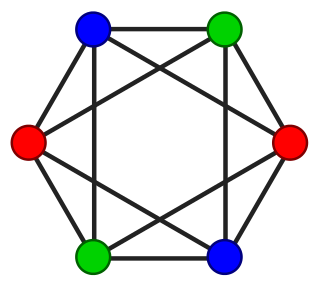
\includegraphics[width=0.5\textwidth]{Images/graphColoring.png}
    \hspace*{\fill}
    \caption{Colorazione di un grafo}
    \label{fig:graphColoring}
\end{figure}
L'idea per realizzare il GA \`e sicuramente pi\`u agevole di quanto abbiamo fatto nel capitolo precedente, ma in certi versi simile: gli operatori fondamentali sono sempre quelli (potremmo agire sulla selezione ed usarne una diversa da quella a torneo, oppure cambiando il crossover), per\`o ci sarebbe il vantaggio di poter usare codifiche di dimensione costante pari al numero di vertici; i cromosomi nascenti da esse avrebbero i geni rappresentanti i colori (o meglio un intero/stringa che identifica univocamente il colore).
\begin{figure}[H]
    \centering
    \hfill
    
\includegraphics[width=0.95\textwidth]{Images/coloring.png}
    \hspace*{\fill}
    \caption{Codifica di un possibile individuo, ad ogni intero corrisponde un colore}
    \label{fig:coloring}
\end{figure}
Viene naturale pensare alla funzione di fitness come alla somma, per ogni cromosoma, dei vertici adiacenti aventi lo stesso colore assegnato; di conseguenza i migliori cromosomi hanno valori di fitness minori rispetto agli altri, per tale ragione l'implementazione ed il ragionamento da eseguire combacia quasi perfettamente con quanto visto per la ricerca del cammino minimo.
\vspace{3mm}

%\textbf{da inserire: codice delle funzioni cardine e commenti}
%
Abbiamo implementato anche noi stessi un algoritmo volto alla colorazione dei grafi, ponendo le fondamenta su quanto fatto da \cite{graphcol1}, ovvero usando il GA fino ad un arbitrario numero di iterazioni per poi concludere con un algoritmo ad hoc (\textit{wisdom of artificial crowds}) in modo da ridurre il margine di errore. Il codice risulta avere la stessa strutture di quanto implementato nel capitolo 4, di fatto non riporteremo il sorgente in appendice, ma spenderemo comunque qualche parola sulle nostre scelte implementative.
\vspace{3mm}

La creazione della prima generazione, a differenza per il problema del cammino minimo, \`e completamente casuale: questo ci permette di avere una popolazione pi\`u ampia e, di conseguenza, maggiori probabilit\`a di raggiungere il risultato ottimale. Dato che i cromosomi hanno dimensione fissa (pari al numero di nodi del grafo), non dobbiamo eseguire controlli ulteriori nell'operatore di selezione e nella mutazione (cosa che ci ha creato non pochi problemi nella ricerca del cammino minimo).
\vspace{3mm}

Gli operatori di selezione, crossover e mutazione rimangono pressoch\'e invariati rispetto a quanto osservato nel capitolo passato; la selezione ed il crossover rimangono, rispettivamente, nella loro variante a torneo ed a punto singolo (senza il bisogno di eliminare nodi duplicati), mentre la mutazione viene enormemente semplificata: scelto casualmente un gene con probabilit\`a \textit{pMutation}, tale operatore non fa altro che impostare il valore del gene ad uno degli altri colori possibili, rendendolo estremamente pi\`u veloce di quanto fatto nel capitolo 4.
\vspace{3mm}

Non ci resta, dunque, che introdurre una possibile funzione di fitness, la quale \`e stata gi\`a in parte descritta in un paragrafo precedente: abbiamo deciso che la funzione sia data dalla somma fra il numero di archi che connettono vertici aventi lo stesso colore assegnato (l'operazione prevede lo scorrimento del cromosoma e l'uso di una matrice di adiacenza) ed il numero di colori usati dal cromosoma.
\vspace{3mm}

\begin{Large}
{$$f(x)=\sum_{i=0}^{|V|-2}(\sum_{j=i+1}^{|V|-1}k)+\#used\_colors$$ }
\end{Large}
con k=$\begin{cases}
$1$, & \text{se v[i] e v[j] sono adiacenti e hanno lo stesso colore} \\
$0$, & \text{altrimenti}
\end{cases}$
\vspace{3mm}

Quest'ultimo parametro (\textit{\#used\_colors}) \`e indispensabile altrimenti i cromosomi usanti tutti colori differenti per la colorazione dei nodi risulterebbero decisamente migliori, pur essendo lontani dall'esserlo. La seguente immagine mostra un chiaro esempio in cui questo parametro risulta essere fondamentale.
\begin{figure}[H]%
    \centering
    %\hfill
    \subfloat[Esempio senza collisioni]{{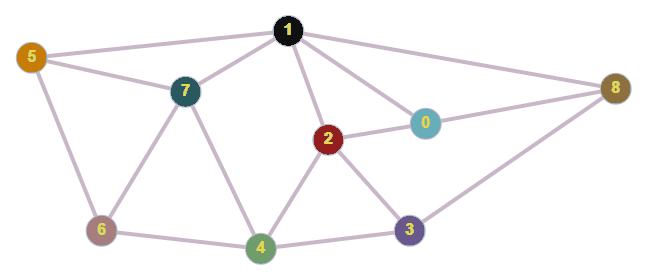
\includegraphics[width=0.5\linewidth]{Images/coloring2.png}}}%
    %\qquad
    %\hfill
    \subfloat[Esempio con collisioni]{{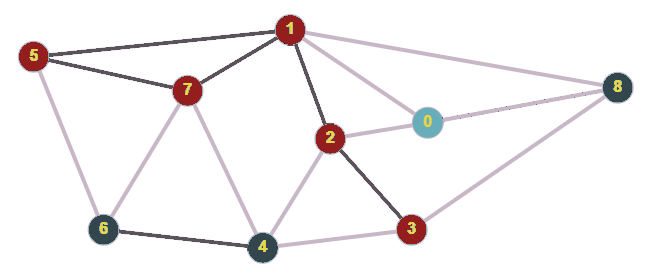
\includegraphics[width=0.5\linewidth]{Images/coloring3.png}}}%
    %\hfill
    %\caption{Confronto fra la prima e l'ultima generazione per la nuova funzione considerata}%
    %\caption{Il problema del commesso viaggiatore, fonte: algorist.com}
    \caption{Due esempi di colorazione di un grafo, il secondo risulta milgiore ai fini della ricerca con un GA}
    \label{fig:coloring2}%
\end{figure}
\vspace{3mm}
Utilizzando la funzione di fitness previamente descritta, possiamo notare come la soluzione proposta a sinistra risulti avere un valore di fitness pari a $9$ derivante solo dai colori usati, mentre la seconda pur avendo la stessa fitness utilizza solamente tre colori; se non avessimo inserito il parametro \textit{\#used\_colors} la prima colorazione sarebbe risultata la migliore in assoluto, ma non avrebbe assolutamente raggiunto $\chi(G)$ e questo avrebbe potuto indurre il nostro algoritmo su una strada sbagliata, pertanto, ai fini della ricerca, la seconda soluzione risulta la migliore per il proseguimento del GA (potremmo, a nostra scelta, eseguire il prodotto fra \textit{\#used\_colors} ed un valore fra 1 e 2, a seconda di quanto desideriamo che tale parametro influisca sul lavoro del nostro algoritmo).
\vspace{3mm}
%Per scelta nostra abbiamo usato lo stesso grafo visto nel capitolo 5 per testare il nostro algoritmo scritto in Java, seppur applicando scelte implementative diverse: la creazione della prima generazione \`e completamente casuale, inoltre vi sono due metodi differenti di mutazione e selezione (uno per quando il valore di fitness risulta molto basso, uno in ogni altro caso \cite{graphcol1}).
%\vspace{3mm}

Il nostro Ga, con le giuste modifiche, risulta avere un potenziale molto elevato dato che il problema della colorazione dei grafi trova le sue applicazioni pratiche in numerevoli campi, fra i quali:
\begin{itemize}
    \item Colorazione delle mappe \cite{graphcol3}.
    \item Scheduling dei processi \cite{graphcol8}.
    \item Allocazione dei registri \cite{graphcol7}.
    \item Ai giochi, caso pi\`u noto \`e sicuramente il sudoku \cite{graphcol2} \cite{graphcol5},
    %di cui daremo una rapida visione per concludere il nostro capitolo.
%\end{itemize}
%Parlando velocemente del sudoku, di cui a nostro parere personale risulta l'esempio pi\`u intuitivo di applicazione della colorazione, possiamo immaginare ogni cella del gioco come un vertice del nostro grafo, ognuno di questi vertici sono connessi a quelli presenti nello stessa quadrante e nella stessa riga/colonna.
%La seguente immagine mostra chiaramente quanti sono gli archi facenti parte del grafo rappresentante le celle del sudoku (blu quelli fra celle dello stesso quadrante, rossi per quelle sulla stessa riga e colonna).
%\vspace{3mm}
    \begin{figure}[H]%
        \centering
        %\hfill
        \subfloat[Sudoku vista 2d]{{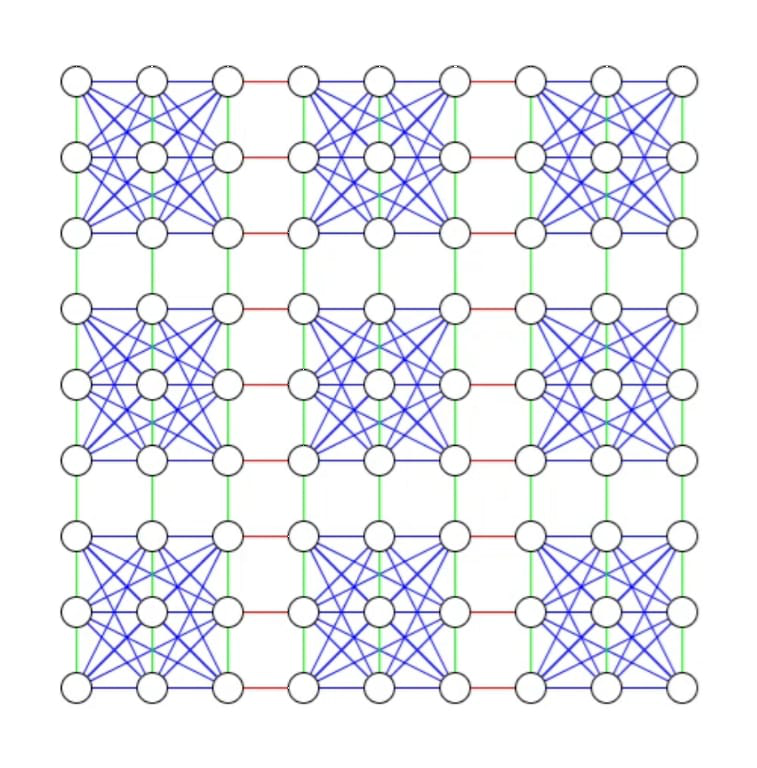
\includegraphics[width=0.5\linewidth]{Images/sudoku2d.png}}}%
        %\qquad
        %\hfill
        \subfloat[Sudoku vista 3d]{{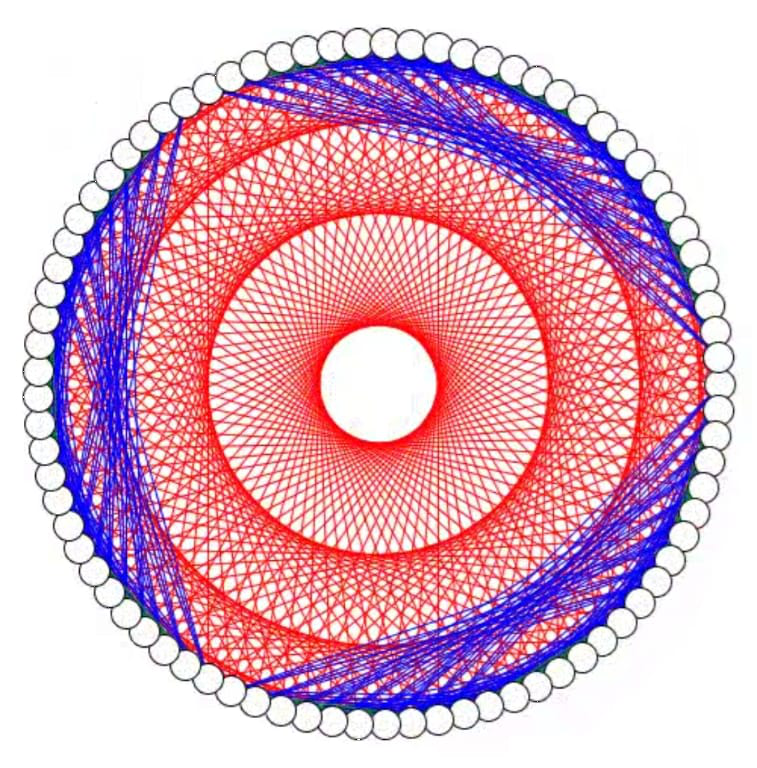
\includegraphics[width=0.5\linewidth]{Images/sudoku3d.png}}}%
        %\hfill
        %\caption{Confronto fra la prima e l'ultima generazione per la nuova funzione considerata}%
        %\caption{Il problema del commesso viaggiatore, immagine trovata dal web}
        \caption{Rappresentazione degli archi del grafo basato sul sudoku}
        \label{fig:sudoku2d3d}%
    \end{figure}
    data la sua predisposizione come strumento di analisi e confronto per gli algoritmi di ricerca.
\end{itemize}
%Considerato che ci sono $9$ quadranti (stesso vale per le righe e colonne), \`e immediato pensare al sudoku come un problema di colorazione con $9$ colori.
%\vspace{3mm}
%\begin{figure}[H]
%    \centering
%    \hfill
%    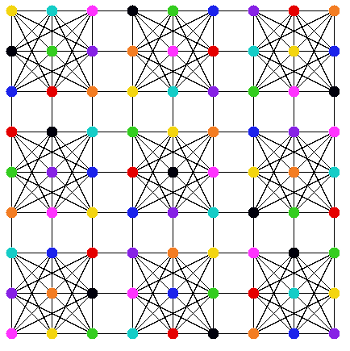
\includegraphics[width=0.50\textwidth]{Images/sudoku.png}
%    \hspace*{\fill}
%    \caption{La colorazione applicata al sudoku, opera di http://www.open-graphtheory.org/}
%    \label{fig:sudoku}
%\end{figure}
%Di fatto, sono state trovate varie soluzioni al gioco del sudoku tramite i GA: se non vogliamo rimanere nell'ambito della colorazione dei grafi, allora vale la pena citare il lavoro eseguito da Mantere e Koljonen \cite{graphcol2} ed ampliato da Deng e Li \cite{graphcol5}, i quali hanno usato un approccio differente (seppur sempre tramite l'uso dei GA) nella creazione e soluzione dei sudoku: non andando nei minimi dettagli, la maggior differenza risiede nella codifica dei cromosomi, i quali non risultano pi\`u essere composti dai colori assegnati ai vertici, ma dai valori delle celle stesse (fra i quali alcuni sono "fissi" ovvero iniziali).
%\vspace{3mm}
%La decisione di prendere in esame rapidamente il sudoku \`e scaturita dal fatto che tale gioco \`e molto noto in ambito scientifico data la sua predisposizione come strumento di test/confronto per gli algoritmi di ricerca, oltre al fatto di essere un buon esempio da suggerire in ambito accademico agli studenti per provare e capire direttamente come lavorare con un GA (abbiamo descritto velocemente due approcci, ma potrebbero sicuramente esisterne altri).
%Oltre ai due casi di esempio portati in questo capitolo, ne esistono sicuramente tantissimi altri, ma abbiamo preferito rimanere legati all'ambito dei grafi per non disorientare troppo il lettore ed appannare le loro idee, d'altronde entrambi gli esempi presenti in queste sezioni sono un piccola goccia in un vasto mare di applicazioni; di questi ne parleremo nel prossimo ed ultimo capitolo.
%La decisione di prendere come esempio rapido il sudoku \`u scaturita dal fatto che tale gioco \`e usato in ambito scientifico per
Dopo aver esposto due ulteriori ambiti di applicazioni dei GA sui grafi, dedicheremo le prossime due sezioni a concludere la tesi, esponendo rapidamente altri campi di utilizzo dei GA, per poi concludere con una piccola riflessione sul loro futuro.
\section{I GA nei vari ambiti scientifici}
Gi\`a Goldman nella sua opera maggiormente nota \cite{goldberg1} inser\`i una esaustiva lista di campi di applicazione dei GA, i diversi ambiti andavano dalla biologia all'informatica, dall'ingegneria meccanica \cite{end1} all'image processing\cite{end2} ed al riconoscimento di pattern \cite{end3}, fino ad arrivare alla finanza\cite{end6} ed alla fisica. Abbiamo sempre ribadito quanto i GA siano flessibili, il loro ampio raggio d'impiego ne \`e la testimonianza pi\`u diretta.
%\vspace{3mm}
\begin{figure}[H]%
    \centering
    %\hfill
    \subfloat[Articoli per anno]{{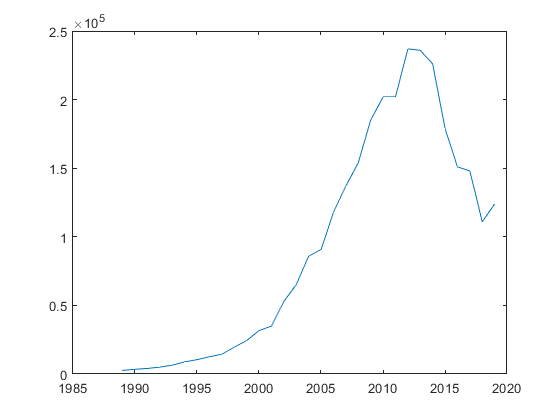
\includegraphics[width=0.5\linewidth]{Images/graph1.png}}}%
    %\qquad
    %\hfill
    \subfloat[Articoli per anno (cumulativi)]{{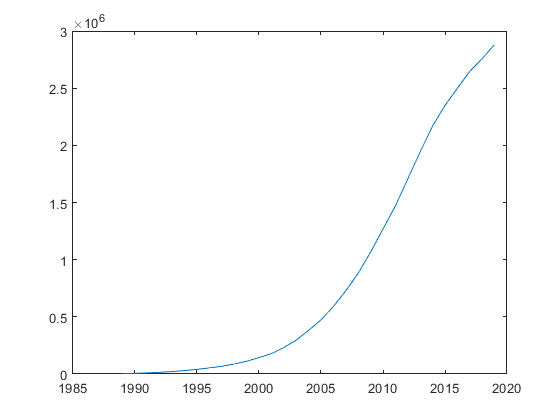
\includegraphics[width=0.5\linewidth]{Images/graph2.png}}}%
    %\hfill
    %\caption{Il problema del commesso viaggiatore, immagine trovata dal web}
    %\caption{Rappresentazione degli archi del grafo basato sul sudoku}
    \caption{Articoli per anno contenenti "Genetic Algorithm", fonte dei dati: Google Scholar}
    \label{fig:articles}%
\end{figure}
Dato il sempre crescente interesse verso il machine learning, i GA stanno ritornando sotto i riflettori anche se Goldberg per primo scrisse chiaramente sul loro uso in tale campo \cite{goldberg1} \cite{end7}; essendo il machine learning \cite{end4} \cite{end5}, e l'IA in generale, l'ambito pi\`u altisonante attualmente unito al sempre maggiore interesse da parte dell'aziende nell'assumere esperti in tali settori, fa comprendere quanto l'approccio mostrato in questa tesi possa risultare un importante tassello per chi prender\`a questa strada.
\section{Conclusioni e visioni sul futuro}
Per quanto ci possa addolarare affermare quanto segue dopo interi capitoli, dobbiamo senza dubbio ammettere che i GA non sono, allo stato attuale e dopo aver visto qualche implementazione, la soluzione migliore per i problemi di ricerca ed ottimizzazione; d'altro canto, abbiamo visto come la loro flessibilit\`a possa dare un grande vantaggio in certe situazioni (come sottolineato verso la fine del capitolo 5, risultano pi\`u efficaci in casi in cui il tempo sia il maggior discriminante).
\vspace{3mm}

Come il loro nome pu\`o suggerire, i GA sono sempre in continua evoluzione e, con la nostra piena speranza, usciranno pubblicazioni negli anni a venire che daranno nuove linfa vitale a questo metodo, la cui idea fondamentale rimane in ogni modo affascinante ed interessante.
%\section{I GA nei vari ambiti scientifici}
%\section{Conclusioni e visioni sul futuro}
\newpage
%
\myChapter{Riflessioni e conclusioni sui GA}
Quest'ultimo capitolo, volto a concludere la tesi, elenca rapidamente alcuni ambiti di applicazione dei GA, per poi terminare con una breve visione su quanto essi potranno essere utili in un futuro prossimo.
\section{I GA nei vari ambiti scientifici}
Gi\`a Goldman nella sua opera maggiormente nota \cite{goldberg1} inser\`i una esaustiva lista di campi di applicazione dei GA, i diversi ambiti andavano dalla biologia all'informatica, dall'ingegneria meccanica \cite{end1} all'image processing\cite{end2} ed al riconoscimento di pattern \cite{end3}, fino ad arrivare alla finanza\cite{end6} ed alla fisica. Abbiamo sempre ribadito quanto i GA siano flessibili, il loro ampio raggio d'impiego ne \`e la testimonianza pi\`u diretta.
%\vspace{3mm}
\begin{figure}[H]%
    \centering
    %\hfill
    \subfloat[Articoli per anno]{{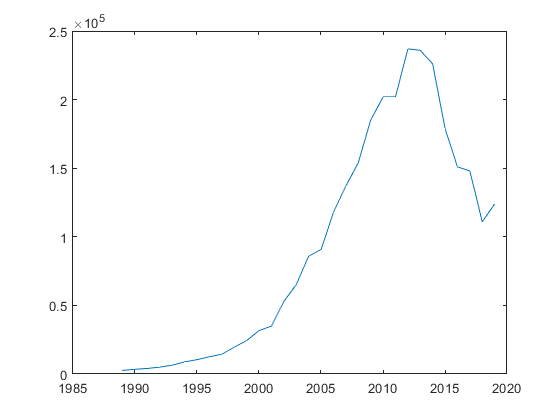
\includegraphics[width=0.5\linewidth]{Images/graph1.png}}}%
    %\qquad
    %\hfill
    \subfloat[Articoli per anno (cumulativi)]{{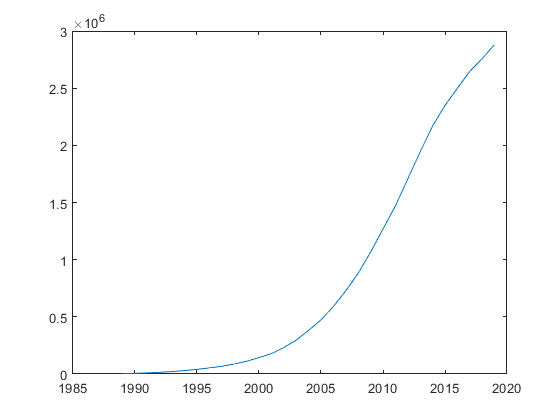
\includegraphics[width=0.5\linewidth]{Images/graph2.png}}}%
    %\hfill
    %\caption{Il problema del commesso viaggiatore, immagine trovata dal web}
    %\caption{Rappresentazione degli archi del grafo basato sul sudoku}
    \caption{Articoli per anno contenenti "Genetic Algorithm", fonte dei dati: Google Scholar}
    \label{fig:articles}%
\end{figure}
Dato il sempre crescente interesse verso il machine learning, i GA stanno ritornando sotto i riflettori anche se Goldberg per primo scrisse chiaramente sul loro uso in tale campo \cite{goldberg1} \cite{end7}; essendo il machine learning \cite{end4} \cite{end5}, e l'IA in generale, l'ambito pi\`u altisonante attualmente unito al sempre maggiore interesse da parte dell'aziende nell'assumere esperti in tali settori, fa comprendere quanto l'approccio mostrato in questa tesi possa risultare un importante tassello per chi prender\`a questa strada.
\section{Conclusioni e visioni sul futuro}
Per quanto ci possa addolarare affermare quanto segue dopo interi capitoli, dobbiamo senza dubbio ammettere che i GA non sono, allo stato attuale e dopo aver visto qualche implementazione, la soluzione migliore per i problemi di ricerca ed ottimizzazione; d'altro canto, abbiamo visto come la loro flessibilit\`a possa dare un grande vantaggio in certe situazioni (come sottolineato verso la fine del capitolo 5, risultano pi\`u efficaci in casi in cui il tempo sia il maggior discriminante).
\vspace{3mm}

Come il loro nome pu\`o suggerire, i GA sono sempre in continua evoluzione e, con la nostra piena speranza, usciranno pubblicazioni negli anni a venire che daranno nuove linfa vitale a questo metodo, la cui idea fondamentale rimane in ogni modo affascinante ed interessante.
%I GA non sono sicuramente, allo stato attuale, il miglior agloritmo in circolazione per quanto riguarda la ricerca e l'ott
%\section{}
\newpage

\myChapter{Ringraziamenti}
Posso dire, in tutta sincerit\`a, che ho cambiato pi\`u volte questo ultimo capitolo, vuoi perch\'e non sono mai stato bravo a scrivere dei veri ringraziamenti, vuoi perch\'e le persone che mi hanno dato una mano durante tutto l'arco di questi anni sono veramente tante (e ricordaserle tutte non \`e affatto banale), ma comunque prover\`o a porgere il mio "grazie" tutti.
\vspace{3mm}

Desidero ringraziare, prima su tutti, la professoressa Verri per la pazienza e la professionalit\`a che mi ha mostrato durante tutto l'arco del tirocinio, oltre al fatto di avermi supportato (posso dire anche sopportato le mie tante domane ed i miei peggiori errori di battitura) nella stesura della tesi.
\vspace{3mm}

Ringrazio la mia famiglia, dai membri pi\`u piccoli che con la loro pura spensieratezza mi hanno dato vigore e strappato qualche sorriso, ai pi\`u "vecchiotti" che mi hanno sempre mostrato quale fosse la realt\`a della vita (sopratutto nel mondo del lavoro e dello studio) ed affrontarla senza timore.
\vspace{3mm}

Altri ringraziamenti vanno ai conoscenti ed agli amici di sempre che mi hanno sempre incoraggiato a portare termine questo cammino iniziato con tante speranze e che sta terminando portandomi nuovi sogni.
\vspace{3mm}

Un immenso "grazie" ai miei colleghi di universit\`a con cui ho condiviso fatiche, gioie ed un'innumerevole quantit\`a di progetti che ci hanno reso pi\`u coesi nell'affrontare ogni esame; la ragione per cui ho potuto passare serenamente, seppur in mezzo a tanti problemi di salute, questi anni \`e anche merito vostro.
\vspace{3mm}

Per ultimo, ringrazio la mia testardaggine che nei momenti di difficolt\`a (vuoi un esame andato non come voluto od i tantissimi problemi avuti in questi tre anni e mezzo) mi obbligava a non darmi per vinto e la mia curiosit\`a, la quale ogni volta riesce sempre a farmi capire quanto ancora ho da scoprire nel campo, l'informatica, che da sempre \`e mi accompagna dandomi ogni volta nuovi stimoli per migliorare.
\newpage

\appendix
\myChapter{Codici}
\section{Capitolo 3}
\subsection{Launcher}
\begin{lstlisting}[style=matlab, style=matlab2, style=matlab3]
x=[0.00:0.01:10.23]';
n=length(x);
y=zeros(n, 1);
y(1:n)=(x(1:n)-7).^2+1; %funzione da minimizzare

popSize=30; %dimensione della popolazione
pCrossover=0.75; %coefficiente di crossover
pMutation=0.0333; %coefficiente di mutazione
maxGen=500; %generazione massima

%popolazione iniziale generata casualmente
p=fix(x(n).*rand(popSize,1)*100)/100;

%inizializzazione e calcolo fitness inziale
fitness=zeros(popSize, 1);
fitness(1:popSize)=(p(1:popSize)-7).^2+1;

%# di generazione in cui il fitness non cambia
cFit=0;

[minFit, minIndex]=min(fitness);
minPoint=p(minIndex);
for i=1:maxGen
    %stampa a video
    fprintf("Generazione: %d, Individuo migliore: %d, 
        Fitness minima: %d, Fitness media: %d\n", i, 
        minPoint, minFit, mean(fitness));
    
    [z,fitness]=GAMatlab(pCrossover,pMutation,p,
        fitness);
    if min(fitness)>=minFit
        cFit=cFit+1;
    else
        [minFit, minIndex]=min(fitness);
        minPoint=z(minIndex);
        cFit=0;
    end
    population=z;
    if cFit==100
        fprintf("Limite massimo raggiunto");
        %potremmo usare un metodo tradizionale
        break; 
    end
end
\end{lstlisting}
\subsection{Function principale ed operatori}
\begin{lstlisting}[style=matlab, style=matlab2, style=matlab3]
function [newPopulation,fitness]=GAMatlab(pCrossover,
pMutation,p,fitness)
%
% [newPopulation,fitness]=GAMatlab(pCrossover,
% pMutation,population,fitness)
% Genera la nuova popolazione attraverso gli
% operatori fondamentali dei GA
n=length(population);
chromosomes=zeros(n,10); 
newChromosomes=zeros(n,10);
newPopulation=zeros(n,1);
k=1; %numero individui della nuova generazione
[fitMin,minIndex]=min(fitness); %fitness minimo
for i=1:n
    %codifica
    chromosomes(i,1:10)=encode(p(i));
end
while k<n+1
    %selezione
    [parent1,chromosomes2,j]=selection(chromosomes,
        fitness);
    fitness2=fitness([1:j-1 j+1:end]);
    parent2=selection(chromosomes2,fitness2);
   
    %crossover
    if (rand(1)<=pCrossover)
        [son1,son2]=crossover(parent1,parent2);
        
        %mutazione
        son1=mutation(pMutation, son1);
        son2=mutation(pMutation, son2);
        
        %aggiunta all'insieme dei nuovi cromosomi
        newChromosomes(k,1:10)=son1;
        newChromosomes(k+1,1:10)=son2;
        k=k+2;
    end
end
for i=1:n
    %decodifica
    newPopulation(i)=decode(newChromosomes(i,1:10));
end
%calcolo del fitness della nuova popolazione
fitness(1:n)=(newPopulation(1:n)-7).^2+1;

%inserisco il miglior individuo della precedente
%generazione al posto del peggiore di quella attuale
[fitMax, maxIndex]=max(fitness);
newPopulation(maxIndex)=p(minIndex);
fitness(maxIndex)=fitMin;
end

%
%Selezione a roulette
%
function [parent,chromosomes2,j]=
    selection(chromosomes,fitness)
sumFit=sum(fitness(1:length(fitness)));
n=length(chromosomes);
partSumFit=0; %somma delle parti
i=1;
randomPoint=rand(1)*sumFit; %numero casuale
while partSumFit<randomPoint && i<n
    partSumFit=partSumFit+fitness(i);
    i=i+1;
end
parent=zeros(1, 10);
parent=chromosomes(i, 1:10);
if nargout>1
    chromosomes2=chromosomes([1:i-1 i+1:end], 1:10);
    j=i;
end
end

%
%Crossover a punto singolo
%
function [son1,son2]=crossover(parent1,parent2)
son1=zeros(1,10);
son2=zeros(1,10);
crossPoint=randi(9, 1);
son1(1:crossPoint)=parent1(1:crossPoint);
son1(crossPoint+1:end)=parent2(crossPoint+1:end);
son2(1:crossPoint)=parent2(1:crossPoint);
son2(crossPoint+1:end)=parent1(crossPoint+1:end);
end

%
%Mutazione
%
function mutChromosome=mutation(pMutation,chromosome)
for i=1:length(chromosome)
    if rand(1)<=pMutation
        chromosome(i)=1-chromosome(i);
    end
end
mutChromosome=chromosome;
end

%
%Codifica
%
function chromosome=encode(individual)
s=fix(individual*100);
output=zeros(1,10);
i=10;
while s>0
    output(1,i)=mod(s, 2);
    s=fix(s/2);
    i=i-1;
end
chromosome=output;
end

%
%Decodifica
%
function individual=decode(chromosome)
individual=0;
for i=10:-1:1
    individual=individual+chromosome(i)*(2^(10-i));
end
individual=individual*0.01;
end
\end{lstlisting}
\section{Capitolo 4}
\subsection{Classe Node}
\begin{lstlisting}[style=Java]
package geneticalgorithm;

import java.util.LinkedList;
import java.util.HashMap;
import java.util.Iterator;

public class Node {
	private String name;
	private LinkedList<Node> path; //cammino minimo dal nodo iniziale
	private int d; //distanza dal nodo sorgente
	private HashMap<Node, Integer> mapNodes; //nodi adiacenti e loro distanza dal nodo stesso
	private int id; //id del nodo, necessario per la matrice di adiacenza
	private static int lastId=0; //ultimo id nodo salvato
	
	public Node(String name) {
		this.name=name;
		path=new LinkedList<>();
		d=Integer.MAX_VALUE;
		mapNodes=new HashMap<>();
		id=lastId++;
	}
	
	/**
	 * Connette il nodo ad un altro nodo n impostando al tempo stesso il peso dell'arco che li congiunge
	 * @param n
	 * @param distance
	 * @param alreadyConnected
	 */
	public void connectTo(Node n, int distance, boolean alreadyConnected) {
		mapNodes.put(n, distance);
		if (!alreadyConnected) n.connectTo(this, distance, true);
	}
	
	/**
	 * Restituisce tutti i nodi adiacenti a tale nodo
	 * @return una HashMap<Node, Integer> di nodi
	 */
	public HashMap<Node, Integer> getConnectedNodes() {
		return mapNodes;
	}
	
	/**
	 * Restituisce il tragitto per arrivare al nodo, usato nell'algoritmo di Dijkstra
	 * @return un iterator di nodi
	 */
	public Iterator<Node> getPath() {
		return path.iterator();
	}
	
	/**
	 * Aggiunge un nodo al cammino per arrivare al nodo in question
	 * @param itPath
	 * @param n
	 */
	public void addToPath(Iterator<Node> itPath, Node n) {
		path.removeAll(path);
		while (itPath.hasNext()) {
			Node m=itPath.next();
			path.add(m);
		}
		path.add(n);
		//path.add(this);
	}
	
	/**
	 * Imposta la distanza cumulativa dal nodo di partenza
	 * @param d
	 */
	public void setDistance(int d) {
		this.d=d;
	}
	
	public int getDistance() {
		return d;
	}
	
	public String getName() {
		return name;
	}
	
	public int getId() {
		return id;
	}
}
\end{lstlisting}
\subsection{Classe Chromosome}
\begin{lstlisting}[style=Java]
package geneticalgorithm;

import java.util.Iterator;
import java.util.ArrayList;
import java.util.Comparator;

public class Chromosome {
	private ArrayList<Node> genes; //lista dei geni
	private int fitness=Integer.MAX_VALUE; //valore di fitness
	
	public Chromosome() {
		genes=new ArrayList<>();
	}
	
	/**
	 * Imposta i geni del cromosoma a partire da un iteratore
	 * @param genes
	 */
	public Chromosome(Iterator<Node> genes) {
		this.genes=new ArrayList<>();
		while (genes.hasNext()) {
			this.genes.add(genes.next());
		}
	}
	
	/**
	 * Restituisce i geni del cromosoma
	 * @return un iterator di geni, ovvero i nodi del grafo
	 */
	public Iterator<Node> getGenes() {
		return genes.iterator();
	}
	
	public int getFitness() {
		return fitness;
	}
	
	public void setFitness(int fitness) {
		this.fitness=fitness;
	}
	
	public int getSize() {
		return genes.size();
	}
	
	/**
	 * Scorrendo tutta la lista dei geni, controlla se il cromosoma corrisponde ad un altro creato in precedenza,
	 * metodo utilizzato solamente nella costruzione della prima generazione
	 * @param c
	 * @return un valore booleano indicante se il cromosoma ha gli stessi geni di un altro cromosoma
	 */
	public boolean hasSamePath(Chromosome c) {
		boolean b=true;
		if (genes.size()==c.getSize()) {
			Iterator<Node> itGenes1=c.getGenes();
			Iterator<Node> itGenes2=getGenes();
			while (itGenes1.hasNext()) {
				Node n1=itGenes1.next();
				Node n2=itGenes2.next();
				if (!n1.equals(n2)) b=false;
			}
			//for(Node)
		} else {
			b=false;
		}
		return b;
	}
	
	@Override
	public String toString() {
		String s="";
		for (Node n: genes) {
			s+=n.getName()+" ";
		}
		return s;
	}
	
	public static Comparator<Chromosome> fitnessComparator = new Comparator<Chromosome>() {
		@Override
		public int compare(Chromosome c1, Chromosome c2) {
			return (c1.getFitness()<c2.getFitness() ? -1 : (c1.getFitness()==c2.getFitness() ? 0 : 1));
		}
	};
 }
\end{lstlisting}
\subsection{Classe Graph}
\begin{lstlisting}[style=Java]
package geneticalgorithm;

import java.util.ArrayList;
import java.util.Iterator;
import java.util.HashMap;
import java.util.Map.Entry;
import java.util.Random;

public class Graph {
	private ArrayList<Node> nodes; //nodi del grafo
	private Population population;
	
	public Graph() {
		nodes=new ArrayList<>();
	}
	
	/**
	 * Aggiunge nodi al grafo
	 * @param n
	 * @throws Exception
	 */
	public void addNode(Node... n) throws Exception{
		for (Node m: n) {
			for (Node k: nodes) {
				if (k.equals(m)) throw new Exception("Il nodo appartiene gi\u00E0 al grafo");
			}
			nodes.add(m);
		}
	}
	
	/**
	 * Partendo da una lista di nodi, restituisce quello con valore di distanza minimo
	 */
	private Node minDistanceNode(ArrayList<Node> nvNodes) {
		Node minNode=null;
		int minDistance=Integer.MAX_VALUE;
		for (Node n: nvNodes) {
			int d=n.getDistance();
			if (d<minDistance) {
				minDistance=d;
				minNode=n;
			}
		}
		return minNode;
	}
	
	/**
	 * Imposta la distanza del nodo destinazione ad un nuovo valore se e solo se
	 * quello precedente risulta maggiore della somma fra l'intero dato passato
	 * come argomento e la distanza cumulativa del nodo destinazione stesso
	 * @param destination
	 * @param source
	 * @param distance
	 */
	private void setDistance(Node destination, Node source, int distance) {
		int sDistance=source.getDistance();
		if (sDistance+distance< destination.getDistance()) {
			destination.setDistance(sDistance+ distance);
			Iterator<Node> path=source.getPath();
			destination.addToPath(path, source);
		}
	}
	
	/**
	 * Calcola il cammino minimo utilizzando l'algoritmo di Dijkstra a partire da un nodo
	 * inziiale verso uno finale
	 * @param source
	 * @param destination
	 * @return il cammino minimo da sorgente a destinazione
	 * @throws Exception
	 */
	public Iterator<Node> DijkstraAlgorithm(Node source, Node destination) throws Exception{
		if (!nodes.contains(source) || !nodes.contains(destination)) throw new Exception("Il nodo definito come iniziale o finale non appartiene al grafo");
		
		//Passo 1 e 2
		source.setDistance(0);
		ArrayList<Node> vNodes=new ArrayList<>();
		ArrayList<Node> nvNodes=new ArrayList<>();
		nvNodes.add(source);
		
		while (nvNodes.size()!=0) {
			Node n=minDistanceNode(nvNodes);
			nvNodes.remove(n);
			if (n.equals(destination)) break; //se siamo giunti a destinazione terminiamo, Passo 5
			
			HashMap<Node, Integer> map=n.getConnectedNodes();
			
			//Passo 3
			for (Entry<Node, Integer> e: map.entrySet()) {
				Node m=e.getKey();
				if (vNodes.contains(m)) continue; //necessaria per grafi non orientati
				int d=e.getValue().intValue();
				//if (!nvNodes.contains(m)) {
					setDistance(m, n, d);
					nvNodes.add(m);
				//}
			}
			
			//Passo 4
			vNodes.add(n);
		}
		return destination.getPath();
	}
	
	/**
	 * Crea un cammino casuale da sorgente a destinazione
	 * @param source
	 * @param destination
	 * @return un iteratore di nodi contenente il cammino casuale
	 */
	public Iterator<Node> createRandomPath(Node source, Node destination) {
		boolean dest=false;
		//ArrayList<Node> nvNodes=nodes.forEach();
		ArrayList<Node> path=new ArrayList<>();
		path.add(source);
		ArrayList<Node> vNodes=new ArrayList<>();
		vNodes.add(source);
		while (dest==false) {
			Node n=path.get(path.size()-1);
			HashMap<Node, Integer> map=n.getConnectedNodes();
			ArrayList<Node> connNodes=new ArrayList<>();
			map.entrySet().forEach(e -> connNodes.add(e.getKey()));
			connNodes.removeIf(k -> vNodes.contains(k));
			if (connNodes.isEmpty()) {
				path.remove(n);
				continue;
			}
			Random r=new Random();
			int randomIndex= r.nextInt(connNodes.size());
			Node m=connNodes.get(randomIndex);
			if (m.equals(destination)) dest=true;
			path.add(m);
			vNodes.add(m);
		}
		return path.iterator();
	}
	
	/**
	 * Calcola il cammino minimo da sorgente a destinazione usando il GA
	 * @param source
	 * @param destination
	 * @param pSize
	 * @param maxGen
	 * @param pCrossover
	 * @param pMutation
	 * @return il cromosoma migliore dell'ultima generazione
	 * @throws Exception
	 */
	public Chromosome ShortestPathGA(Node source, Node destination, int pSize, int maxGen, double pCrossover, double pMutation) throws Exception{
		if (nodes.size()==0) throw new Exception("Non sono stati inseriti nodi nel grafo");
		
		//Creo la popolazione e costruisco la matrice di adiacenza
		population=new Population(nodes.size(), pSize, this);
		population.buildMatrixDist(nodes.iterator());
		
		int j=0;
		while (j<pSize) {
			//Creo un cromosoma assegnandoli un percorso (geni) casuale fra sorgente e destinazione
			Chromosome c=new Chromosome(createRandomPath (source, destination));
			Iterator<Chromosome> itC=population.getChromosomes();
			
			//Controllo se tale percorso esiste già
			boolean hasSamePath=false;
			while (itC.hasNext()) {
				if (itC.next(). hasSamePath(c)) {
					hasSamePath=true;
					break;
				}
			}
			if (!hasSamePath) {
				//Nel caso il cromosoma fosse unico (percorso differente dagli altri), lo aggiungo alla popolazione
				population.addChromosome(c);
				j++;
			}
		}
		
		//Eseguo il GA per un numero massimo di generazioni
		for (int i=0;i<maxGen; i++) {
			population.pathGA(pCrossover, pMutation);
		}
		return population.getFittest(); //Restituzione del miglior cromosoma
	}
}
\end{lstlisting}
\subsection{Classe Population}
\begin{lstlisting}[style=Java]
package geneticalgorithm;

import java.util.ArrayList;
import java.util.Collections;
import java.util.Iterator;
import java.util.HashMap;
import java.util.Map.Entry;
import java.util.Random;
import java.util.stream.Collectors;

public class Population {
	private ArrayList<Chromosome> chromosomes;
	private int bestFitness=Integer.MAX_VALUE; //miglior valore di fitness
	private Chromosome best=null; //miglior individuo
	private int[][] matDist; //matrice delle distanze
	private int pSize; //dimensione popolazione
	private Graph graph;
	private int nCrossover=0; //numero di crossover
	private int nMutation=0; //numero di mutazioni
	
	public Population(int size, int pSize, Graph graph) {
		chromosomes=new ArrayList<>();
		matDist=new int[size][size];
		for (int i=0;i<matDist.length;i++) {
			for (int j=0;j<matDist.length;j++) {
				matDist[i][j]=100;
			}
		}
		this.pSize=pSize;
		this.graph=graph;
	}
	
	/**
	 * Aggiunge un cromosoma alla popolazione
	 * @param c
	 */
	public void addChromosome(Chromosome c) {
		chromosomes.add(c);
		setFitness(c);
	}
	
	/**
	 * Imposta il valore di fitness di un cromosoma
	 * @param c
	 */
	private void setFitness(Chromosome c) {
		int fitness=0;
		Iterator<Node> itNodes=c.getGenes();
		int idPrev=itNodes.next().getId();
		while (itNodes.hasNext()) {
			int idNext=itNodes.next().getId();
			fitness+=matDist[idPrev][idNext];
			idPrev=idNext;
		}
		c.setFitness(fitness);
	}
	
	/**
	 * Restituisce il cromosoma con il miglior valore di fitness
	 * @return il cromosoma migliore
	 */
	public Chromosome getFittest() {
		return best;
	}
	
	/**
	 * Costruisce la matrice di adiacenza
	 * @param itNodes
	 */
	public void buildMatrixDist(Iterator<Node> itNodes) {
		while (itNodes.hasNext()) {
			Node n=itNodes.next();
			HashMap<Node, Integer> map=n.getConnectedNodes();
			int idN=n.getId();
			for (Entry<Node, Integer> e: map.entrySet()) {
				Node m=e.getKey();
				int dist= e.getValue().intValue();
				int idM=m.getId();
				if (matDist[idN][idM]==100) {
					matDist[idN][idM]= dist;
					matDist[idM][idN]= dist;
				}
			}
		}
	}
	
	/**
	 * Operatore di selezione, applica la sua variante a torneo
	 * @return due cromosomi genitori
	 */
	private ArrayList<Chromosome> selection() {
		//Dimensione del torneo
		int tSize=5;
		
		//Lista temporanea dei cromosomi
		ArrayList<Chromosome> tChroms=new ArrayList<>();
		
		chromosomes.forEach(c -> tChroms.add(c));
		Random r=new Random();
		
		//Cromosomi genitori
		ArrayList<Chromosome> parents=new ArrayList<>();
		
		while (parents.size()<2) {
			//Cromosomi partecipanti al torneo
			ArrayList<Chromosome> selChroms=new ArrayList<>();
			while (selChroms.size()<tSize) {
				int rInt= r.nextInt(tChroms.size());
				Chromosome c=tChroms.get(rInt);
				if (!selChroms.contains(c)) {
					selChroms.add(c);
				}
			}
			
			Collections.sort(selChroms, Chromosome.fitnessComparator);
			
			//Scelta del vincitore del torneo
			double p=0.75;
			double[] partialSums=new double[tSize];
			double sumP=0;
			for (int i=0;i<tSize;i++) {
				sumP+=p*Math.pow((1-p), i);
				partialSums[i]=sumP;
			}
			double rDouble=r.nextDouble()*sumP;
			int i=0;
			while (partialSums[i]<rDouble) {
				i++;
			}
			parents.add(selChroms.get(i));
			tChroms.remove(i);
		}
		return parents;
	}
	
	/**
	 * Operatore di crossover, nella sua variante a punto singolo
	 * @param parents
	 * @return una lista contenente i geni dei figli
	 */
	private ArrayList<ArrayList<Node>> crossover(ArrayList<Chromosome> parents) {
		//Estrazione dei due genitori dalla lista
		Chromosome parent1=parents.get(0);
		Chromosome parent2=parents.get(1);
		
		ArrayList<Node> son1=new ArrayList<>();
		ArrayList<Node> son2=new ArrayList<>();
		
		//Ottenimento dei geni dei due genitori
		Iterator<Node> itP1=parent1.getGenes();
		Iterator<Node> itP2=parent2.getGenes();
		
		//Calcolo della dimensione minima
		int minSize=parent1.getSize();
		if (parent2.getSize()<minSize) minSize=parent2.getSize();
		
		//Generazione del punto di crossover
		Random r=new Random();
		int rIndex=r.nextInt(minSize-1);
		
		//Crossover a punto singolo
		int i=0;
		while (i<rIndex) {
			son1.add(itP1.next());
			son2.add(itP2.next());
			i++;
		}
		while (itP1.hasNext()) {
			son2.add(itP1.next());
		}
		while (itP2.hasNext()) {
			son1.add(itP2.next());
		}
		
		//Restituzione dei due figli
		ArrayList<ArrayList<Node>> sons=new ArrayList<>();
		sons.add(son1);
		sons.add(son2);
		return sons;
	}
	
	/**
	 * Operatore di mutazione
	 * @param individuals
	 * @param pMutation
	 */
	private void mutation(ArrayList<ArrayList<Node>> individuals, double pMutation) {
		Random r=new Random();
		for (int i=0;i<individuals.size();i++) {
			ArrayList<Node> son=individuals.get(i);
			for (int j=0;j<son.size()-1;j++) {
				double rDouble=r.nextDouble();
				
				//Se la mutazione avviene, trovo un nuovo percorso dal nodo scelto verso la destinazione
				if (rDouble<pMutation) {
					nMutation++;
					Node n=son.get(j);
					Iterator<Node> itN= graph. createRandomPath(n, son.get (son.size()-1));
					
					//Eliminimo gli elementi successivi al nodo che ha subito la mutazione
					for (int k= son.size()-1;k>= j;k--) {
						son.remove(k);
					}
					
					//Aggiungo il percorso
					while (itN.hasNext()) son.add(itN.next());
					break;
				}
			}
			
			//Elimino i nodi dupilcati
			son=(ArrayList<Node>)son.stream() .distinct().collect(Collectors. toList());
		}
	}
	
	/**
	 * Creazione della nuova generazione attraverso i tre operatori fondamentali
	 * @param pCrossover
	 * @param pMutation
	 */
	public void pathGA(double pCrossover, double pMutation) {
		ArrayList<Chromosome> newGeneration=new ArrayList<>();
		while (newGeneration.size()<pSize) {
			//Selezione
			ArrayList<Chromosome> parents=selection();
			
			//Generazione di un numero casuale fra 0 ed 1
			Random r=new Random();
			double rDouble=r.nextDouble();
			
			//Crossover
			if (rDouble<pCrossover) {
				nCrossover++;
				ArrayList<ArrayList<Node>> sons=crossover(parents);
				
				//Mutazione
				mutation(sons, pMutation);
				
				//Aggiunta dei nuovi cromosomi alla popolazione
				newGeneration.add(new Chromosome(sons. get(0).iterator()));
				newGeneration.add(new Chromosome(sons. get(1).iterator()));
				
			}
		}
		newGeneration.forEach(c -> setFitness(c));
		Collections.sort(newGeneration, Chromosome.fitnessComparator);
		int i=newGeneration.size()-1;
		while (newGeneration.size()>pSize) {
			newGeneration.remove(i);
			i--;
		}
		chromosomes=newGeneration;
		best=chromosomes.get(0);
		bestFitness=best.getFitness();
	}
	
	@Override
	public String toString() {
		String s="";
		for (Chromosome c: chromosomes) {
			s+=c.toString()+" fitness: "+c.getFitness()+"\n";
		}
		return s;
	}
	
	public int getBestFitness() {
		return bestFitness;
	}
	
	public String getStats() {
		String s="Numero di crossover: "+nCrossover+", numero di mutazioni: "+nMutation;
		return s;
	}
	
	public Iterator<Chromosome> getChromosomes() {
		return chromosomes.iterator();
	}
}
\end{lstlisting}
%\section{Capitolo 5}
\newpage
%\begin{thebibliography}{99}

\bibitem{goldberg1}{D. E. Goldberg - \emph{Genetic Algorithms in Search, Optimization \& Machine Learning} - Addison-Wesley, 1989}

\bibitem{selection1}{B. L. Miller, D. E. Goldberg - \emph{Genetic Algorithms, Tournament Selection, and the Effects of Noise} - Complex Systems, 9, 1995, Pages 193-212}

\bibitem{selection2}{R. Sivaraj, T. Ravichandran - \emph{A Rewiew of Selection Methods In Genetic Algorithm}}

\bibitem{glossary}{Thomas Baeck, D.B Fogel, Z Michalewicz - \emph{Evolutionary Computation 1: Basic Algorithms and Operators}}

\bibitem{path1}{Tony White, Bernard Pagurek, Franz Oppacher1 - \emph{ASGA: Improving the Ant System by Integration with Genetic
Algorithms} - altre informazioni}

\bibitem{path2}{Sachith Abeysundara, Baladasan Giritharan, Saluka Kodithuwakku - \emph{A Genetic Algorithm Approach to Solve the
Shortest Path Problem for Road Maps}}

\bibitem{path3}{Bilal Gonen - \emph{Genetic Algorithm Finding the Shortest Path in Networks}}

\bibitem{path4}{Yinzhen Li, Ruichun He, Yaohuang Guo - \emph{Faster Genetic Algorithm for Network Paths}}

\bibitem{tsp1}{Michael J\"unger, Gerhard Reinelt, Giovanni Rinaldi - \emph{Handbooks in Operations Research and Management Science} - Volume 7, 1995, Pages 225-330}

\bibitem{tsp2}{Heinrich Braun - \emph{On solving travelling salesman problems by genetic algorithms}}

\bibitem{tsp3}{H. M\"uhlenbein, M. Gorges-Schleuter, O. Kr\"amer - \emph{Evolution algorithms in combinatorial optimization} - Volume 7, Issue 1, April 1988, Pages 65-85}

\bibitem{tsp4}{Noraini Mohd Razali, John Geraghty
 - \emph{Genetic Algorithm Performance with Different
Selection Strategies in Solving TSP}}

\bibitem{tsp5}{P. Larranaga, C. M. H. Kuijpers, R. H. Murga, I. Inza, S. Dizdarevic - \emph{Genetic Algorithms for the Travelling Salesman Problem: A Review of Representations and Operators} -  Artificial Intelligence Review 13, 1999, Pages 129-170}

\bibitem{path5}{K. De Jong, W. M. Spears - \emph{Using Genetic Algorithms to Solve NP Complete Problems} - Proceedings of the Third International Conference on Genetic Algorithm, Morgan Kaufman, Los Altos, CA, 1989, Pages 124-132}

\bibitem{graphcol1}{Musa M. Hindi, Roman V. Yampolskiy - \emph{Genetic Algorithm Applied to the Graph Coloring Problem}}

\bibitem{graphcol4}{Josephine Yik Chong Leung, Wai Shan Lui - \emph{The Application of Graph Theory to Sudoku} - Hang Lung Mathematics Awards, 2014, Vol. 6}

\bibitem{graphcol2}{Timo Mantere, Janne Koljonen - \emph{Solving, rating and Generating Sudoku Puzzles with GA}}

\bibitem{graphcol3}{Bah-Hwee Gwee, Josep S. Chang - \emph{A hybrid genetic hill-climbing algorithm for four-coloring map problems} - Design and application of hybrid intelligent systems, 2003, Pages 252-261}

\bibitem{graphcol5}{Xiu Qin Deng, Yong Da Li - \emph{A novel hybrid genetic algorithm for solving Sudoku puzzles}}

\bibitem{graphcol6}{Charles Fleurent, Jacques A. Ferland - \emph{Genetic and hybrid algorithms for graph coloring} - Annals of Operations Research, June 1996, Volume 63, Issue 3, Pages 437-461}

\bibitem{end1}{H. Khayyam, A. Jamali, H. Assimi, R. N. Jazar (2020) - \emph{Genetic Programming Approaches in Design and Optimization of Mechanical Engineering Applications} - Nonlinear Approaches in Engineering Application, 2019, Pages 367-402}

\bibitem{end2}{Seyedali Mirjalil, Jin Song Dong, Ali Safa Sadiq, Hossam Faris - \emph{Genetic Algorithm: Theory, Literature Review, and Application in Image Reconstruction} - Nature-Inspired Optimizers, 2019, Pages 69-85}

\bibitem{end3}{S. K. Pal, P. P. Wang - \emph{Genetic algorithms for pattern recognition}}

\bibitem{end4}{John J. Grefenstette - \emph{Genetic Algorithms and Machine Learning}}

\bibitem{end5}{Haleh Vafaie, Kenneth De Jong
 - \emph{Genetic Algorithms as a Tool for Feature Selection in Machine Learning}}
 
\bibitem{end6}{Robert Pereira - \emph{Genetic Algorithm Optimisation for Finance and Investment} - 2000}

%\bibitem{graphcol5}{ - \emph{}}

%\bibitem{graphcol4}{ - \emph{}}

%\bibitem{tsp2}{}

\end{thebibliography}

\bibliographystyle{unsrt}
\bibliography{Chapters/references}
%--------------------------------------------------------------
\end{document}
%--------------------------------------------------------------
